\documentclass[11pt,compress,t,notes=noshow, xcolor=table]{beamer}

% graphicx and color are loaded via lmu-lecture.sty
% maxwidth is the original width if it is less than linewidth
% otherwise use linewidth (to make sure the graphics do not exceed the margin)
% TODO: Remove once cleared to be superfluous
% \makeatletter
% \def\maxwidth{ %
%   \ifdim\Gin@nat@width>\linewidth
%     \linewidth
%   \else
%     \Gin@nat@width
%   \fi
% }
% \makeatother

% ---------------------------------%
% latex-math dependencies, do not remove:
% - mathtools
% - bm
% - siunitx
% - dsfont
% - xspace
% ---------------------------------%

%--------------------------------------------------------%
%       Language, encoding, typography
%--------------------------------------------------------%

\usepackage[english]{babel}
\usepackage[utf8]{inputenc} % Enables inputting UTF-8 symbols
% Standard AMS suite (loaded via lmu-lecture.sty)

% Font for double-stroke / blackboard letters for sets of numbers (N, R, ...)
% Distribution name is "doublestroke"
% According to https://mirror.physik.tu-berlin.de/pub/CTAN/fonts/doublestroke/dsdoc.pdf
% the "bbm" package does a similar thing and may be superfluous.
% Required for latex-math
\usepackage{dsfont}

% bbm – "Blackboard-style" cm fonts (https://www.ctan.org/pkg/bbm)
% Used to be in common.tex, loaded directly after this file
% Maybe superfluous given dsfont is loaded
% TODO: Check if really unused?
% \usepackage{bbm}

% bm – Access bold symbols in maths mode - https://ctan.org/pkg/bm
% Required for latex-math, preferred over \boldsymbol
% https://tex.stackexchange.com/questions/3238/bm-package-versus-boldsymbol
\usepackage{bm}

% pifont – Access to PostScript standard Symbol and Dingbats fonts
% Used for \newcommand{\xmark}{\ding{55}, which is never used
% aside from lecture_advml/attic/xx-automl/slides.Rnw
% \usepackage{pifont}

% Quotes (inline and display), provdes \enquote
% https://ctan.org/pkg/csquotes
\usepackage{csquotes}

% Adds arg to enumerate env, technically superseded by enumitem according
% to https://ctan.org/pkg/enumerate
% Replace with https://ctan.org/pkg/enumitem ?
% Even better: enumitem is not really compatible with beamer and breaks all sorts of things
% particularly the enumerate environment. The enumerate package also just isn't required
% from what I can tell so... don't re-add it I guess?
% \usepackage{enumerate}

% Line spacing - provides \singlespacing \doublespacing \onehalfspacing
% https://ctan.org/pkg/setspace
% \usepackage{setspace}

% mathtools – Mathematical tools to use with amsmath
% https://ctan.org/pkg/mathtools?lang=en
% latex-math dependency according to latex-math repo
\usepackage{mathtools}

% Maybe not great to use this https://tex.stackexchange.com/a/197/19093
% Use align instead -- TODO: Global search & replace to check, eqnarray is used a lot
% $ rg -f -u "\begin{eqnarray" -l | grep -v attic | awk -F '/' '{print $1}' | sort | uniq -c
%   13 lecture_advml
%   14 lecture_i2ml
%    2 lecture_iml
%   27 lecture_optimization
%   45 lecture_sl
\usepackage{eqnarray}
% For shaded regions / boxes
% Used sometimes in optim
% https://www.ctan.org/pkg/framed
\usepackage{framed}

%--------------------------------------------------------%
%       Cite button (version 2024-05)
%--------------------------------------------------------%

% Superseded by style/ref-buttons.sty, kept just in case these don't work out somehow.

% Note this requires biber to be in $PATH when running,
% telltale error in log would be e.g. Package biblatex Info: ... file 'authoryear.dbx' not found
% aside from obvious "biber: command not found" or similar.
% Tried moving this to lmu-lecture.sty but had issues I didn't quite understood,
% so it's here for now.

\usepackage{hyperref}

% Only try adding a references file if it exists, otherwise
% this would compile error when references.bib is not found
% NOTE: Bibliography packages (usebib, biblatex) are now loaded by ref-buttons.sty when needed
% This keeps all bibliography-related setup in one place

% Legacy \citelink command removed - superseded by ref-buttons.sty

%--------------------------------------------------------%
%       Displaying code and algorithms
%--------------------------------------------------------%

% Reimplements verbatim environments: https://ctan.org/pkg/verbatim
% verbatim used sed at least once in
% supervised-classification/slides-classification-tasks.tex
% Removed since code should not be put on slides anyway
% \usepackage{verbatim}

% Both used together for algorithm typesetting, see also overleaf: https://www.overleaf.com/learn/latex/Algorithms
% algorithmic env is also used, but part of the bundle:
%   "algpseudocode is part of the algorithmicx bundle, it gives you an improved version of algorithmic besides providing some other features"
% According to https://tex.stackexchange.com/questions/229355/algorithm-algorithmic-algorithmicx-algorithm2e-algpseudocode-confused
\usepackage{algorithm}
\usepackage{algpseudocode}

%--------------------------------------------------------%
%       Tables
%--------------------------------------------------------%

% multi-row table cells: https://www.namsu.de/Extra/pakete/Multirow.html
% Provides \multirow
% Used e.g. in evaluation/slides-evaluation-measures-classification.tex
\usepackage{multirow}

% colortbl: https://ctan.org/pkg/colortbl
% "The package allows rows and columns to be coloured, and even individual cells." well.
% Provides \columncolor and \rowcolor
% \rowcolor is used multiple times, e.g. in knn/slides-knn.tex
\usepackage{colortbl}

% long/multi-page tables: https://texdoc.org/serve/longtable.pdf/0
% Not used in slides
% \usepackage{longtable}

% pretty table env: https://ctan.org/pkg/booktabs
% Is used
% Defines \toprule
\usepackage{booktabs}

%--------------------------------------------------------%
%       Figures: Creating, placing, verbing
%--------------------------------------------------------%

% wrapfig - Wrapping text around figures https://de.overleaf.com/learn/latex/Wrapping_text_around_figures
% Provides wrapfigure environment -used in lecture_optimization
\usepackage{wrapfig}

% Sub figures in figures and tables
% https://ctan.org/pkg/subfig -- supersedes subfigure package
% Provides \subfigure
% \subfigure not used in slides but slides-tuning-practical.pdf errors without this pkg, error due to \captionsetup undefined
\usepackage{subfig}

% Actually it's pronounced PGF https://en.wikibooks.org/wiki/LaTeX/PGF/TikZ
\usepackage{tikz}

% No idea what/why these settings are what they are but I assume they're there on purpose
\usetikzlibrary{shapes,arrows,automata,positioning,calc,chains,trees, shadows}
\tikzset{
  %Define standard arrow tip
  >=stealth',
  %Define style for boxes
  punkt/.style={
    rectangle,
    rounded corners,
    draw=black, very thick,
    text width=6.5em,
    minimum height=2em,
    text centered},
  % Define arrow style
  pil/.style={
    ->,
    thick,
    shorten <=2pt,
    shorten >=2pt,}
}


% textpos package to allow absolute placement of environments like figures
% See e.g. https://datumorphism.leima.is/til/programming/latex-beamer-textblock-position/
%  - absolute: Enables absolute positioning mode where coordinates are measured from the top-left corner of the page/frame, rather than relative to the current text position.
%  - overlay: Makes the positioned content behave as an overlay that doesn't affect the normal text flow or spacing. Without this, positioned elements could interfere with the document's layout.
% 
%   The \textblock* environment creates a text block at absolute coordinates:
% 
%   \begin{textblock*}{\linewidth}(0cm,4cm) % (x,y) from top-left of frame
%     \imageC[1]{figure/cov_funs/cov_matern.pdf}
%   \end{textblock*}
\usepackage[absolute,overlay]{textpos}

%--------------------------------------------------------%
%       Beamer setup and custom macros & environments
%--------------------------------------------------------%

% Main sty file for beamer setup (layout, style, lecture page numbering, etc.)
% For long-term maintenance, this may me refactored into a more modular set of .sty files
\usepackage{../../style/lmu-lecture-new}
% Custom itemize wrappers, itemizeS, itemizeL, etc

% Used regularly
\let\code=\texttt

% Not sure what/why this does
\setkeys{Gin}{width=0.9\textwidth}

% -- knitr leftovers --
% These may be used by knitr/R Markdown workflows in other lectures
\makeatletter
\def\maxwidth{ %
  \ifdim\Gin@nat@width>\linewidth
    \linewidth
  \else
    \Gin@nat@width
  \fi
}
\makeatother

% Define colors for syntax highlighting (may be used by knitr)
\definecolor{fgcolor}{rgb}{0.345, 0.345, 0.345}
\definecolor{shadecolor}{rgb}{.97, .97, .97}

% knitr code output environment
\newenvironment{knitrout}{}{}

\newcommand{\citebutton}[2]{%
\beamergotobutton{\href{#2}{#1}}%
}

\newcommand{\ques}{\textbf{\textcolor{red}{Question:  }}}
\newcommand{\questionssofar}{\begin{frame}\frametitle{Any questions?}\end{frame}}

\newcommand\warning{%
 \makebox[1.4em][c]{%
 \makebox[0pt][c]{\raisebox{.1em}{\scriptsize!}}%
 \makebox[0pt][c]{\color{red}\normalsize$\bigtriangleup$}}}%

% Can't find a reason why common.tex is not just part of this file?
% This file is included in slides and exercises

% Rarely used fontstyle for R packages, used only in 
% - forests/slides-forests-benchmark.tex
% - exercises/single-exercises/methods_l_1.Rnw
% - slides/cart/attic/slides_extra_trees.Rnw
\newcommand{\pkg}[1]{{\fontseries{b}\selectfont #1}}

% Spacing helpers, used often (mostly in exercises for \dlz)
\newcommand{\lz}{\vspace{0.5cm}} % vertical space (used often in slides)
\newcommand{\dlz}{\vspace{1cm}}  % double vertical space (used often in exercises, never in slides)
\newcommand{\oneliner}[1] % Oneliner for important statements, used e.g. in iml, algods
{\begin{block}{}\begin{center}\begin{Large}#1\end{Large}\end{center}\end{block}}

% Don't know if this is used or needed, remove?
% textcolor that works in mathmode
% https://tex.stackexchange.com/a/261480
% Used e.g. in forests/slides-forests-bagging.tex
% [...] \textcolor{blue}{\tfrac{1}{M}\sum^M_{m} [...]
% \makeatletter
% \renewcommand*{\@textcolor}[3]{%
%   \protect\leavevmode
%   \begingroup
%     \color#1{#2}#3%
%   \endgroup
% }
% \makeatother



% custom packages
\usepackage{subfig}
\usepackage{psfrag}
\usepackage{algorithm}
\usepackage{algpseudocode}
\usepackage{eqnarray}
\usepackage{arydshln}
\usepackage{tabularx}
\usepackage{placeins}
\usepackage{tikz}
\usepackage{setspace}
\usepackage{colortbl}
\usepackage{mathtools}
\usepackage{wrapfig}
\usepackage{listings}

\usepackage{framed}
\makeatletter
\newenvironment{kframe}{%
 \def\at@end@of@kframe{}%
 \ifinner\ifhmode%
  \def\at@end@of@kframe{\end{minipage}}%
  \begin{minipage}{\columnwidth}%
 \fi\fi%
 \def\FrameCommand##1{\hskip\@totalleftmargin \hskip-\fboxsep
 \colorbox{shadecolor}{##1}\hskip-\fboxsep
     % There is no \\@totalrightmargin, so:
     \hskip-\linewidth \hskip-\@totalleftmargin \hskip\columnwidth}%
 \MakeFramed {\advance\hsize-\width
   \@totalleftmargin\z@ \linewidth\hsize
   \@setminipage}}%
 {\par\unskip\endMakeFramed%
 \at@end@of@kframe}
\makeatother

\usepackage{tcolorbox}
\usepackage{dsfont}
\usepackage{tikz}

\definecolor{texblue}{rgb}{0, 0, 1}
\def\myblue#1{\textcolor{texblue}{#1}}

% Notation carried over from the tokenization lecture
\newcommand{\vocab}{\mathcal{V}}
\newcommand{\probs}{\boldsymbol{\phi}}

% Generic notation for deep latent variable models (following Luo, 2022)
\providecommand{\bx}{\mathbf{x}}
\providecommand{\bz}{\mathbf{z}}



\tikzset{
  invisible/.style={opacity=0, text opacity=0},
  visible on/.style={alt={#1{}{invisible}}},
  alt/.code args={<#1>#2#3}{\alt<#1>{\pgfkeysalso{#2}}{\pgfkeysalso{#3}}},
  % graphical models
  gm latent/.style={circle, draw, thick, minimum size=8mm, inner sep=0pt},
  gm obs/.style={gm latent, fill=black!12},
  gm param/.style={circle, fill, inner sep=1.3pt},
  gm gen/.style={->, thick},
  gm inf/.style={->, thick, dashed, draw=texblue},
  gm lab/.style={font=\scriptsize, inner sep=2pt},
  pf pt/.style={circle, fill=#1, inner sep=1.6pt},
  pf seq/.style={font=\footnotesize, text=#1, anchor=south, inner sep=2pt},
  pf num/.style={font=\scriptsize, text=#1, inner sep=1pt},
  pf map/.style={->, thick, draw=#1, shorten <=2pt, shorten >=2pt},
  pf fibre/.style={rounded corners=4pt, fill=#1!7, draw=#1!40},
  pf post/.style={font=\scriptsize, text=#1, fill=white, draw=#1!40, rounded corners=2pt, inner sep=1.5pt},
}

% Run bibliography entries together instead of breaking after each block
\setbeamertemplate{bibliography entry title}{}
\setbeamertemplate{bibliography entry location}{}
\setbeamertemplate{bibliography entry note}{}

% Numbered labels [1], [2] instead of the little paper icon
\setbeamertemplate{bibliography item}{\insertbiblabel}

% ToC
\AtBeginSection[]{
	\begin{frame}[noframenumbering, plain]
	\frametitle{Outline}
	\setcounter{tocdepth}{1}
	\tableofcontents[currentsection]
\end{frame}
}

\title{Deep Learning for NLP II}

\begin{document}

\titlemeta{
Diffusion Language Models
}{}{
figure/diffusion-title.png
}{
\item Deep latent variable models
\item Diffusion models as Markovian hierarchical VAEs
\item Masked diffusion language models
}

% ------------------------------------------------------------------------------


\begin{frame}{Diffusion LLMs in Action}
 
\def\eostok{{\ttfamily\scriptsize<eos>}}
 
\vfill
 
\begin{center}
\begin{tikzpicture}[
  cell/.style={rounded corners=2pt, minimum width=1.3cm, minimum height=0.7cm, text height=1.6ex, text depth=0.4ex, inner sep=1pt, thick, font=\footnotesize},
  masked/.style={cell, fill=black!8, draw=black!25, text=black!45, font=\scriptsize\ttfamily},
  fresh/.style={cell, fill=blue!12, draw=blue!70, text=blue!70!black},
  done/.style={cell, fill=white, draw=black!35},
]
 
  % ---- prompt (conditioning, never masked) ----------------------------------
  \node[anchor=west, font=\small, fill=black!4, draw=black!15, rounded corners=3pt, inner sep=4pt]
    at (-0.65,1.5) {\textbf{Prompt:} \textit{What is a diffusion LM? Answer in one sentence.}};
 
  \node[anchor=west, font=\footnotesize\bfseries] at (-0.65,0.65) {Response:};
 
  % ---- response canvas: 21 positions, 7 per row -----------------------------
  \foreach \tok/\s [count=\i from 0] in {
      A/2, diffusion/1, LM/1, starts/3, from/3, fully/6, masked/2,
      text/3, and/4, unmasks/3, many/6, tokens/2, in/4, parallel/4,
      {,}/5, step/4, by/5, step/2, ./1, \eostok/1, \eostok/1} {
    \pgfmathtruncatemacro{\col}{mod(\i,7)}
    \pgfmathtruncatemacro{\row}{div(\i,7)}
    \pgfmathtruncatemacro{\fr}{\s+1}
    \pgfmathtruncatemacro{\dn}{\s+2}
    \only<1-\s>{\node[masked] at (\col*1.42, -\row*0.95) {[MASK]};}
    \only<\fr>{\node[fresh] at (\col*1.42, -\row*0.95) {\tok};}
    \only<\dn->{\node[done] at (\col*1.42, -\row*0.95) {\tok};}
  }
 
\end{tikzpicture}
\end{center}
 
\vfill
 
\uncover<8->{\centering \Large \textbf{What do you observe?}\par}
 
\vfill

\end{frame}




\begin{frame}{Outline}
\tableofcontents
\end{frame}

\section{Deep Latent Variable Models}

\begin{frame}{Recap: Unigram Latent Variable Model}


\vfill
 
\begin{itemize}
\item Observed variable $\mathbf{S}$ (string), latent variable $\mathbf{V}$ (segmentation)
\item Prior over segmentations: $P(\mathbf{V} = \mathbf{v}; \probs) = \prod_{t=1}^{|\mathbf{v}|} \phi_{v_t}$
\item Deterministic likelihood: $P(\mathbf{S} = \mathbf{s} \mid \mathbf{V} = \mathbf{v}) = \mathds{1}[g(\mathbf{v}) = \mathbf{s}]$
\item Marginal (pushforward): $P(\mathbf{S} = \mathbf{s}; \probs) = \sum_{\mathbf{v} \in \mathcal{T}_{\vocab}(\mathbf{s})} P(\mathbf{V} = \mathbf{v}; \probs)$
\item Posterior for $\mathbf{v} \in \mathcal{T}_{\vocab}(\mathbf{s})$ (Bayes' rule):
\begin{equation*}
P(\mathbf{V} = \mathbf{v} \mid \mathbf{S} = \mathbf{s}; \probs) = \frac{P(\mathbf{V} = \mathbf{v}; \probs)}{P(\mathbf{S} = \mathbf{s}; \probs)}
\end{equation*}
\end{itemize}
 
\vfill
 

\end{frame}




\begin{frame}{Recap: EM for Unigram}
 
\vfill
 
\begin{itemize}
\item Goal: maximize the observed data log-likelihood $\log P(\mathbf{S} = \mathbf{s}; \probs)$
\item As a proxy, we maximize the expected complete data log-likelihood $Q(\probs; \probs^{(n)}) =  \sum_{\mathbf{v} \in \mathcal{T}_{\vocab}(\mathbf{s})} P(\mathbf{V} = \mathbf{v} \mid \mathbf{S} = \mathbf{s}; \probs^{(n)}) \log P(\mathbf{V} = \mathbf{v}; \probs)$

\item $\log P(\mathbf{S} = \mathbf{s}; \probs)$ is related to $Q(\probs; \probs^{(n)})$ as follows:
\begin{align*}
\log P(\mathbf{S} = \mathbf{s}; \probs) &= \underbrace{Q(\probs; \probs^{(n)}) + H(\mathbf{V} \mid \mathbf{S} = \mathbf{s}; \probs^{(n)})}_{\text{evidence lower bound (ELBO)}}\\
&\quad + \underbrace{\operatorname{KL}\big(P(\mathbf{V} \mid \mathbf{S} = \mathbf{s}; \probs^{(n)}) \,\big\|\, P(\mathbf{V} \mid \mathbf{S} = \mathbf{s}; \probs)\big)}_{\geq 0;\ 0 \text{ at } \probs = \probs^{(n)}}
\end{align*}
\item \textbf{E-step}: compute the exact posterior $P(\mathbf{V} \mid \mathbf{S} = \mathbf{s}; \probs^{(n)})$ and expected counts with forward-backward
\item \textbf{M-step}: maximize $Q(\probs; \probs^{(n)})$ by normalizing the expected counts
\end{itemize}
 
\vfill
 
\end{frame}




\begin{frame}{Recap: Visualized Example}
 
\colorlet{hl}{orange!85!black}
 
\vfill
 
\begin{center}
\begin{tikzpicture}[x=0.93cm]
  \colorlet{main}{blue}
  \colorlet{other}{black!50}
 
  % ---- preimages T_V(s) (drawn first so they sit behind) --------------------
  \draw[pf fibre=other, visible on=<2->] (0.15,1.55) rectangle (2.65,2.7);
  \draw[pf fibre=main,  visible on=<2->] (3.15,1.55) rectangle (7.45,2.7);
  \draw[pf fibre=other, visible on=<2->] (8.05,1.55) rectangle (8.95,2.7);
  \node[pf num=other, anchor=south, visible on=<2->] at (1.4,2.7)  {$\mathcal{T}_{\vocab}(\textit{ha})$};
  \node[pf num=main,  anchor=south, visible on=<2->] at (5.3,2.7)  {$\mathcal{T}_{\vocab}(\textit{hat})$};
  \node[pf num=other, anchor=south, visible on=<2->] at (8.5,2.7)  {$\mathcal{T}_{\vocab}(\textit{t})$};
 
  % ---- the two spaces -------------------------------------------------------
  \node (Vs) at (-0.55,1.8) {$\vocab^*$};
  \node (Ss) at (-0.55,0)   {$\Sigma^*$};
  \draw[->, thick] (Vs.south) -- node[left] {$g$} (Ss.north);
 
  \draw[thick, black!30] (0,1.8) -- (9.3,1.8) node[right, black!50, font=\small] {$\cdots$};
  \draw[thick, black!30] (0,0)   -- (9.3,0)   node[right, black!50, font=\small] {$\cdots$};
 
  % ---- token sequences with P(V = v; phi) -----------------------------------
  \node[pf pt=other] (v1) at (0.7,1.8) {};
  \node[pf seq=other] (v1l) at (v1.north) {$\langle \texttt{h}, \texttt{a} \rangle$};
  \node[pf num=other, anchor=south] at (v1l.north) {$0.03$};
 
  \node[pf pt=other] (v2) at (2.1,1.8) {};
  \node[pf seq=other] (v2l) at (v2.north) {$\langle \texttt{ha} \rangle$};
  \node[pf num=other, anchor=south] at (v2l.north) {$0.2$};
 
  \node[pf pt=main] (v3) at (3.8,1.8) {};
  \node[pf seq=main] (v3l) at (v3.north) {$\langle \texttt{h}, \texttt{a}, \texttt{t} \rangle$};
  \node[pf num=main, anchor=south] at (v3l.north) {$0.0075$};
 
  \node[pf pt=main] (v4) at (5.3,1.8) {};
  \node[pf seq=main] (v4l) at (v4.north) {$\langle \texttt{ha}, \texttt{t} \rangle$};
  \node[pf num=main, anchor=south] at (v4l.north) {$0.05$};
 
  \node[pf pt=main] (v5) at (6.8,1.8) {};
  \node[pf seq=main] (v5l) at (v5.north) {$\langle \texttt{h}, \texttt{at} \rangle$};
  \node[pf num=main, anchor=south] at (v5l.north) {$0.045$};
 
  \node[pf pt=other] (v6) at (8.5,1.8) {};
  \node[pf seq=other] (v6l) at (v6.north) {$\langle \texttt{t} \rangle$};
  \node[pf num=other, anchor=south] at (v6l.north) {$0.25$};
 
  % ---- strings --------------------------------------------------------------
  \node[pf pt=other] (s1) at (1.4,0) {};
  \node[font=\footnotesize, text=other, anchor=north] (s1l) at (s1.south) {\textit{ha}};
  \node[pf pt=main] (s2) at (5.3,0) {};
  \node[font=\footnotesize, text=main, anchor=north] (s2l) at (s2.south) {\textit{hat}};
  \node[pf pt=other] (s3) at (8.5,0) {};
  \node[font=\footnotesize, text=other, anchor=north] (s3l) at (s3.south) {\textit{t}};
 
  % ---- g: every token sequence goes to exactly one string -------------------
  \draw[pf map=other, visible on=<2->] (v1) -- (s1);
  \draw[pf map=other, visible on=<2->] (v2) -- (s1);
  \draw[pf map=main,  visible on=<2->] (v3) -- (s2);
  \draw[pf map=main,  visible on=<2->] (v4) -- (s2);
  \draw[pf map=main,  visible on=<2->] (v5) -- (s2);
  \draw[pf map=other, visible on=<2->] (v6) -- (s3);
 
  % ---- P(S = s; phi): mass collected from the preimage ----------------------
  \node[pf num=other, anchor=north, visible on=<3->] at (s1l.south) {$0.03 + 0.2 = 0.23$};
  \node[pf num=main,  anchor=north, visible on=<3->] at (s2l.south) {$0.0075 + 0.05 + 0.045 = 0.1025$};
  \node[pf num=other, anchor=north, visible on=<3->] at (s3l.south) {$0.25$};
 
  % ---- posterior P(V = v | S = g(v); phi): renormalize within each preimage --
  \node[pf post=other, visible on=<4->] at (0.7,1.38) {$0.130$};
  \node[pf post=other, visible on=<4->] at (2.1,1.38) {$0.870$};
  \node[pf post=main,  visible on=<4->] at (3.8,1.38) {$0.073$};
  \node[pf post=main,  visible on=<4->] at (5.3,1.38) {$0.488$};
  \node[pf post=main,  visible on=<4->] at (6.8,1.38) {$0.439$};
  \node[pf post=other, visible on=<4->] at (8.5,1.38) {$1$};
 
  % ---- E-step example: posteriors of all segmentations containing h ---------
  \node[pf post=other, draw=hl, very thick, visible on=<5->] at (0.7,1.38) {$0.130$};
  \node[pf post=main,  draw=hl, very thick, visible on=<5->] at (3.8,1.38) {$0.073$};
  \node[pf post=main,  draw=hl, very thick, visible on=<5->] at (6.8,1.38) {$0.439$};
\end{tikzpicture}
\end{center}
 
\vfill

 
\begin{overprint}
\onslide<1-4>
\vfill
\begin{itemize}
\item Prior $P(\mathbf{V} = \mathbf{v}; \probs)$ on top of each token sequence
\item<2-> $g$ maps each token sequence to one string
\item<3-> Marginal: each string collects the mass of its preimage
\item<4-> Posterior: renormalize the prior within each preimage
\end{itemize}
 
\onslide<5-6>
\begin{center}
\footnotesize
\renewcommand{\arraystretch}{1.1}
\begin{tabular}{lcccccc}
$\mathcal{C} = \{\textit{ha}, \textit{hat}, \textit{t}\}$ & \texttt{h} & \texttt{a} & \texttt{t} & \texttt{ha} & \texttt{at} & sum \\
\hline
\rule{0pt}{2.6ex}$\phi^{(n)}_v$ & 0.3 & 0.1 & 0.25 & 0.2 & 0.15 & 1 \\
$\hat{c}_v(\mathcal{C}; \probs^{(n)})$ & \textcolor{hl}{\textbf{0.643}} & 0.204 & 1.561 & 1.357 & 0.439 & 4.204 \\
$\phi^{(n+1)}_v$ & \uncover<6->{\textcolor{hl}{\textbf{0.153}}} & \uncover<6->{0.048} & \uncover<6->{0.371} & \uncover<6->{0.323} & \uncover<6->{0.104} & \uncover<6->{1}
\end{tabular}
\end{center}
\begin{itemize}
\item \textbf{E-step}: $\hat{c}_{\texttt{h}} = 0.130 + 0.073 + 0.439 \approx 0.643$
\item<6-> \textbf{M-step}: $\phi^{(n+1)}_{\texttt{h}} = 0.643 / 4.204 \approx 0.153$
\end{itemize}
\end{overprint}
 
\vfill
 
\end{frame}


\begin{frame}{Notation}
\vfill

\begin{itemize}
\item Shorthand:
\begin{itemize}
\item Observed variable $\bx$, latent variable $\bz$, model parameters $\theta, \phi$
\item $p_\theta(\bx): = P(\mathbf{X} = \bx; \theta)$, and analogously $p_\theta(\bz \mid \bx)$, etc.
\item $p$: probability mass function (discrete) or density (continuous)
\end{itemize}


\item Unigram in this notation:
\begin{equation*}
\bx = \mathbf{s}, \quad \bz = \mathbf{v}, \quad \theta = \probs, \quad p_\theta(\bx \mid \bz) = \mathds{1}[g(\bz) = \bx]
\end{equation*}
\end{itemize}

\vfill

\end{frame}


\begin{frame}{Deep Latent Variable Model Basics}

\vfill

\begin{itemize}
\item In \textbf{deep latent variable models}, $\bz$ captures abstract properties of $\bx$ (e.g., meaning), and a neural network maps $\bz$ to $\bx$
\item Generative story:
\begin{align*}
\bz &\sim p(\bz) && \text{(prior: e.g., } \mathcal{N}(\mathbf{0}, \mathbf{I})\text{)}\\
\bx &\sim p_\theta(\bx \mid \bz) && \text{(likelihood: neural network)}
\end{align*}
\item Marginal likelihood: $p_\theta(\bx) = \int p(\bz)\, p_\theta(\bx \mid \bz)\, d\bz$
\item Same recipe as Unigram (model observed data by marginalizing out the latent), but with much more flexible components
\item Problems:
\begin{itemize}
\item High-dimensional integral over a neural network is intractable
\item Posterior $p_\theta(\bz \mid \bx)$ requires $p_\theta(\bx)$, so it is also intractable $\rightarrow$ we cannot apply EM like for Unigram
\end{itemize}
\end{itemize}

\vfill

\end{frame}


\begin{frame}{ELBO for Deep Latent Variable Models}

\vfill

\begin{itemize}
\item Idea: approximate the intractable posterior by a distribution $q_\phi(\bz \mid \bx)$ from a tractable family (e.g., Gaussians)
\item For \emph{any} such $q_\phi$, we can write (using $\int q_\phi(\bz \mid \bx)\, d\bz = 1$):
\begin{align*}
\log p_\theta(\bx) &= \mathbb{E}_{q_\phi(\bz \mid \bx)}\big[\log p_\theta(\bx)\big]
= \mathbb{E}_{q_\phi(\bz \mid \bx)}\left[\log \frac{p_\theta(\bx, \bz)}{p_\theta(\bz \mid \bx)}\right]\\
&= \mathbb{E}_{q_\phi(\bz \mid \bx)}\left[\log \frac{p_\theta(\bx, \bz)\, q_\phi(\bz \mid \bx)}{p_\theta(\bz \mid \bx)\, q_\phi(\bz \mid \bx)}\right]\\
&= \underbrace{\mathbb{E}_{q_\phi(\bz \mid \bx)}\left[\log \frac{p_\theta(\bx, \bz)}{q_\phi(\bz \mid \bx)}\right]}_{\operatorname{ELBO}(\phi, \theta; \bx)} + \underbrace{\mathbb{E}_{q_\phi(\bz \mid \bx)}\left[\log \frac{q_\phi(\bz \mid \bx)}{p_\theta(\bz \mid \bx)}\right]}_{\operatorname{KL}(q_\phi(\bz \mid \bx) \,\|\, p_\theta(\bz \mid \bx))}
\end{align*}
\item<2-> Connection to last week: splitting the logarithm gives
\begin{equation*}
\operatorname{ELBO}(\phi, \theta; \bx) = \mathbb{E}_{q_\phi(\bz \mid \bx)}\big[\log p_\theta(\bx, \bz)\big] + H\big[q_\phi(\bz \mid \bx)\big]
\end{equation*}
\item<2-> If $q_\phi$ is the Unigram posterior, the first term is exactly $Q$
\end{itemize}

\vfill

\end{frame}


\begin{frame}{Why Maximize the ELBO?}

\vfill

\begin{center}
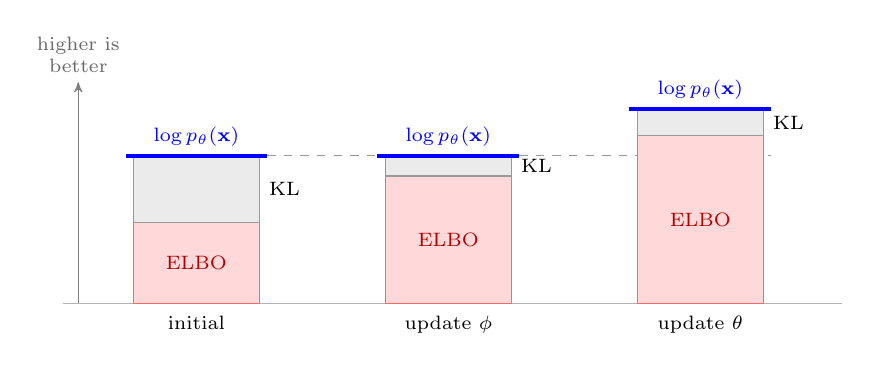
\begin{tikzpicture}[yscale=0.85]
  % axis and baseline
  \draw[->, black!50] (-0.7,0) -- (-0.7,3.3) node[above, font=\scriptsize, text=black!60, align=center] {higher is\\better};
  \draw[black!30] (-0.9,0) -- (9.0,0);

  % ---- initial ---------------------------------------------------------------
  \fill[red!15, draw=red!60] (0,0) rectangle (1.6,1.2);
  \node[font=\scriptsize, text=red!70!black] at (0.8,0.6) {ELBO};
  \fill[black!8, draw=black!40] (0,1.2) rectangle (1.6,2.2);
  \node[font=\scriptsize, anchor=west] at (1.6,1.7) {KL};
  \draw[very thick, blue] (-0.1,2.2) -- (1.7,2.2);
  \node[font=\scriptsize, text=blue, anchor=south] at (0.8,2.2) {$\log p_\theta(\bx)$};
  \node[font=\scriptsize, anchor=north] at (0.8,-0.05) {initial};

  % ---- after maximizing w.r.t. psi -------------------------------------------
  \draw[dashed, black!40, visible on=<2->] (1.7,2.2) -- (4.9,2.2);
  \fill[red!15, draw=red!60, visible on=<2->] (3.2,0) rectangle (4.8,1.9);
  \node[font=\scriptsize, text=red!70!black, visible on=<2->] at (4.0,0.95) {ELBO};
  \fill[black!8, draw=black!40, visible on=<2->] (3.2,1.9) rectangle (4.8,2.2);
  \node[font=\scriptsize, anchor=west, visible on=<2->] at (4.8,2.05) {KL};
  \draw[very thick, blue, visible on=<2->] (3.1,2.2) -- (4.9,2.2);
  \node[font=\scriptsize, text=blue, anchor=south, visible on=<2->] at (4.0,2.2) {$\log p_\theta(\bx)$};
  \node[font=\scriptsize, anchor=north, visible on=<2->] at (4.0,-0.05) {update $\phi$};

  % ---- after maximizing w.r.t. theta -----------------------------------------
  \draw[dashed, black!40, visible on=<3->] (4.9,2.2) -- (8.1,2.2);
  \fill[red!15, draw=red!60, visible on=<3->] (6.4,0) rectangle (8.0,2.5);
  \node[font=\scriptsize, text=red!70!black, visible on=<3->] at (7.2,1.25) {ELBO};
  \fill[black!8, draw=black!40, visible on=<3->] (6.4,2.5) rectangle (8.0,2.9);
  \node[font=\scriptsize, anchor=west, visible on=<3->] at (8.0,2.7) {KL};
  \draw[very thick, blue, visible on=<3->] (6.3,2.9) -- (8.1,2.9);
  \node[font=\scriptsize, text=blue, anchor=south, visible on=<3->] at (7.2,2.9) {$\log p_\theta(\bx)$};
  \node[font=\scriptsize, anchor=north, visible on=<3->] at (7.2,-0.05) {update $\theta$};
\end{tikzpicture}
\end{center}


\begin{itemize}
\item ELBO and KL always add up to $\log p_\theta(\bx)$
\item<2-> $\log p_\theta(\bx)$ does not depend on $\phi$: increasing the ELBO w.r.t.\ $\phi$ must decrease the KL, so $q_\phi$ moves toward the \textbf{true posterior}
\item<3-> Increasing the ELBO w.r.t.\ $\theta$ pushes up a lower bound on $\log p_\theta(\bx)$, so the model improves
%\item<4-> Deep latent variable models maximize the ELBO jointly over $\phi$ and $\theta$ with gradient ascent (\textbf{variational inference})
\end{itemize}

\vfill

\end{frame}



\begin{frame}{Variational Autoencoders (VAEs)}

\vfill

\begin{itemize}
\item Introduced independently by Kingma and Welling (2014) \citebutton{Kingma and Welling (2014)\cite{kingma2014auto}}{https://arxiv.org/abs/1312.6114} and Rezende et al.\ (2014) \citebutton{Rezende et al.\ (2014)\cite{rezende2014stochastic}}{https://proceedings.mlr.press/v32/rezende14.html}
\item Maximize the ELBO jointly over $\phi$ and $\theta$ with gradient ascent
\begin{itemize}
\item \textbf{Encoder} $q_\phi(\bz \mid \bx)$: maps $\bx$ to a distribution over latents
\item \textbf{Decoder} $p_\theta(\bx \mid \bz)$: maps latents back to a distribution over observations
\end{itemize}
\item \textbf{Amortized inference}: VAEs learn a \emph{single} network that outputs $q_\phi(\bz \mid \bx)$ for any $\bx$
\end{itemize}

\vfill

\centering
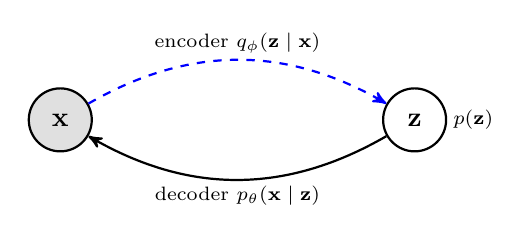
\begin{tikzpicture}
  \node[gm obs] (x) at (0,0) {$\bx$};
  \node[gm latent] (z) at (4.5,0) {$\bz$};
  \draw[gm inf] (x) to[bend left=30] node[gm lab, above] {encoder $q_\phi(\bz \mid \bx)$} (z);
  \draw[gm gen] (z) to[bend left=30] node[gm lab, below] {decoder $p_\theta(\bx \mid \bz)$} (x);
  \node[gm lab, anchor=west] at (z.east) {$p(\bz)$};
\end{tikzpicture}

\vfill

\end{frame}



\begin{frame}{VAE Objective}

\vfill

\begin{itemize}
\item Plugging $p_\theta(\bx, \bz) = p_\theta(\bx \mid \bz)\, p(\bz)$ into $\operatorname{ELBO}(\phi, \theta; \bx)$:
\begin{align*}
\operatorname{ELBO}(\phi, \theta; \bx) &= \mathbb{E}_{q_\phi(\bz \mid \bx)}\left[\log \frac{p_\theta(\bx \mid \bz)\, p(\bz)}{q_\phi(\bz \mid \bx)}\right]\\
&= \mathbb{E}_{q_\phi(\bz \mid \bx)}\big[\log p_\theta(\bx \mid \bz)\big] + \mathbb{E}_{q_\phi(\bz \mid \bx)}\left[\log \frac{p(\bz)}{q_\phi(\bz \mid \bx)}\right]\\
&= \underbrace{\mathbb{E}_{q_\phi(\bz \mid \bx)}\big[\log p_\theta(\bx \mid \bz)\big]}_{\text{reconstruction term}} - \underbrace{\operatorname{KL}\big(q_\phi(\bz \mid \bx) \,\|\, p(\bz)\big)}_{\text{prior matching term}}
\end{align*}
\item \textbf{Reconstruction term}: latents sampled from the encoder should allow the decoder to regenerate $\bx$
\item \textbf{Prior matching term}: the encoder should not stray too far from the prior (why?)
\end{itemize}

\vfill

\end{frame}


\begin{frame}{Standard Choices for VAEs}

\vfill

\begin{itemize}
\item Prior: $p(\bz) = \mathcal{N}(\bz; \mathbf{0}, \mathbf{I})$
\item Encoder: Gaussian with diagonal covariance
\begin{equation*}
q_\phi(\bz \mid \bx) = \mathcal{N}\big(\bz; \boldsymbol{\mu}_\phi(\bx), \operatorname{diag}(\boldsymbol{\sigma}^2_\phi(\bx))\big)
\end{equation*}
\item These choices make prior matching term computable analytically
\item Reconstruction term: Monte Carlo estimate with $\bz^{(l)} \sim q_\phi(\bz \mid \bx)$
\begin{equation*}
\mathbb{E}_{q_\phi(\bz \mid \bx)}\big[\log p_\theta(\bx \mid \bz)\big] \approx \frac{1}{L} \sum_{l=1}^{L} \log p_\theta(\bx \mid \bz^{(l)})
\end{equation*}
\item \textbf{Reparameterization trick}: since we cannot backpropagate into $\phi$ through a sampling step, we write the sample as a deterministic function of $\phi$ and parameter-free noise:
\begin{equation*}
\bz = \bz_\phi(\boldsymbol{\epsilon}) := \boldsymbol{\mu}_\phi(\bx) + \boldsymbol{\sigma}_\phi(\bx) \odot \boldsymbol{\epsilon}, \qquad \boldsymbol{\epsilon} \sim \mathcal{N}(\mathbf{0}, \mathbf{I})
\end{equation*}
\item Randomness now sits in $\boldsymbol{\epsilon}$, so gradients flow through $\boldsymbol{\mu}_\phi$ and $\boldsymbol{\sigma}_\phi$
\end{itemize}

\vfill

\end{frame}

\begin{frame}{Putting the VAE Together}
 
\vfill
 
\begin{center}
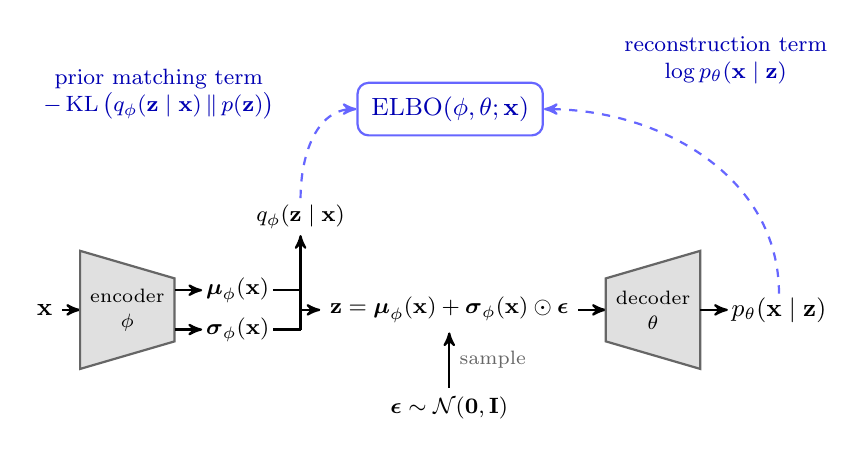
\begin{tikzpicture}[
  net/.style={fill=black!12, draw=black!60, thick},
  arr/.style={->, thick},
  lossarr/.style={->, thick, dashed, draw=blue!60},
  losstxt/.style={font=\footnotesize, text=blue!70!black, align=center},
]
  % ---- input and encoder ------------------------------------------------------
  \node[font=\small] (x) at (0.1,0) {$\bx$};
  \draw[arr] (x.east) -- (0.55,0);
  \draw[net] (0.55,-0.75) -- (1.75,-0.4) -- (1.75,0.4) -- (0.55,0.75) -- cycle;
  \node[font=\scriptsize, align=center] at (1.15,0) {encoder\\[1pt]$\phi$};
 
  % ---- encoder outputs and approximate posterior ------------------------------
  \draw[arr] (1.75,0.25) -- (2.1,0.25) node[right, font=\footnotesize, inner sep=1pt] (mu) {$\boldsymbol{\mu}_\phi(\bx)$};
  \draw[arr] (1.75,-0.25) -- (2.1,-0.25) node[right, font=\footnotesize, inner sep=1pt] (sig) {$\boldsymbol{\sigma}_\phi(\bx)$};
  \draw[thick] (mu.east) -- (3.35,0.25);
  \draw[thick] (sig.east) -- (3.35,-0.25);
  \draw[thick] (3.35,-0.25) -- (3.35,0.25);
  \draw[arr] (3.35,0.25) -- (3.35,0.95) node[above, font=\footnotesize, inner sep=2pt] (q) {$q_\phi(\bz \mid \bx)$};
 
  % ---- reparameterized sample -------------------------------------------------
  \node[anchor=west, font=\footnotesize] (z) at (3.6,0) {$\bz = \boldsymbol{\mu}_\phi(\bx) + \boldsymbol{\sigma}_\phi(\bx) \odot \boldsymbol{\epsilon}$};
  \draw[arr] (3.35,0) -- (z.west);
  \path (z.south) ++(0,-0.7) node[anchor=north, font=\footnotesize] (eps) {$\boldsymbol{\epsilon} \sim \mathcal{N}(\mathbf{0}, \mathbf{I})$};
  \draw[arr] (eps.north) -- node[right, font=\scriptsize, text=black!60] {sample} (z.south);
 
  % ---- decoder and output -----------------------------------------------------
  \draw[arr] (z.east) -- ++(0.35,0) coordinate (din);
  \draw[net] (din) ++(0,-0.4) -- ++(1.2,-0.35) -- ++(0,1.5) -- ++(-1.2,-0.35) -- cycle;
  \path (din) ++(0.6,0) node[font=\scriptsize, align=center] {decoder\\[1pt]$\theta$};
  \draw[arr] (din) ++(1.2,0) -- ++(0.35,0) node[right, inner sep=1pt, font=\small] (out) {$p_\theta(\bx \mid \bz)$};
 
  % ---- loss -------------------------------------------------------------------
  \node[draw=blue!60, thick, rounded corners=4pt, inner sep=5pt, font=\small, text=blue!70!black] (elbo) at (5.25,2.55) {$\operatorname{ELBO}(\phi, \theta; \bx)$};
 
  \node[losstxt, anchor=south] (kl) at (1.55,2.3) {prior matching term\\$-\operatorname{KL}\big(q_\phi(\bz \mid \bx) \,\|\, p(\bz)\big)$};
  \node[losstxt, anchor=south] (rec) at (8.75,2.75) {reconstruction term\\$\log p_\theta(\bx \mid \bz)$};
 
  \draw[lossarr] (q.north) to[out=90, in=180] (elbo.west);
  \draw[lossarr] (out.north) to[out=90, in=0] (elbo.east);
\end{tikzpicture}
\end{center}
  
\begin{itemize}
\item Training: encode, sample via reparameterization, decode, and maximize the ELBO w.r.t.\ $\phi$ and $\theta$ (SGD)
\item Generation: drop the encoder, sample $\bz \sim p(\bz)$, and decode
\end{itemize}
 
\vfill
 
 
\end{frame}



\begin{frame}{Hierarchical VAEs}

\vfill

\begin{itemize}
\item Idea: several levels of latents $\bz_1, \dots, \bz_T$, with higher levels encoding more abstract properties \citebutton{Vahdat and Kautz (2020)\cite{vahdat2020nvae}}{https://arxiv.org/abs/2007.03898}


\item In a general hierarchical VAE (HVAE), each latent may condition on all previous latents
\item \textbf{Markovian HVAE}: the process is a Markov chain, so each latent depends only on the one directly before it
\item Intuitively, a Markovian HVAE is a stack of VAEs
\end{itemize}

\vfill

\centering
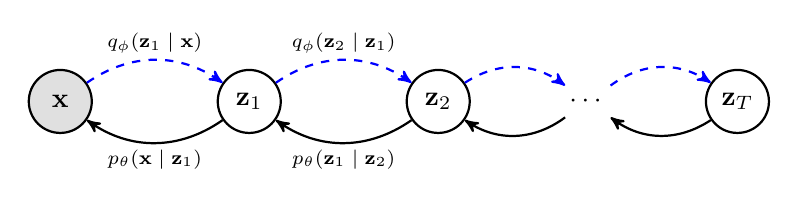
\begin{tikzpicture}
  \node[gm obs]    (x)  at (0,0)   {$\bx$};
  \node[gm latent] (z1) at (2.4,0) {$\bz_1$};
  \node[gm latent] (z2) at (4.8,0) {$\bz_2$};
  \node            (zd) at (6.7,0) {$\cdots$};
  \node[gm latent] (zT) at (8.6,0) {$\bz_T$};

  % encoder (inference), drawn above
  \draw[gm inf] (x)  to[bend left=35] node[gm lab, above] {$q_\phi(\bz_1 \mid \bx)$} (z1);
  \draw[gm inf] (z1) to[bend left=35] node[gm lab, above] {$q_\phi(\bz_2 \mid \bz_1)$} (z2);
  \draw[gm inf] (z2) to[bend left=35] (zd);
  \draw[gm inf] (zd) to[bend left=35] (zT);

  % decoder (generation), drawn below
  \draw[gm gen] (z1) to[bend left=35] node[gm lab, below] {$p_\theta(\bx \mid \bz_1)$} (x);
  \draw[gm gen] (z2) to[bend left=35] node[gm lab, below] {$p_\theta(\bz_1 \mid \bz_2)$} (z1);
  \draw[gm gen] (zd) to[bend left=35] (z2);
  \draw[gm gen] (zT) to[bend left=35] (zd);
\end{tikzpicture}

\vfill

\end{frame}


\begin{frame}{Markovian HVAEs}

\vfill

\begin{itemize}
\item Joint distribution ($\bz_T \to \dots \to \bz_1 \to \bx$):
\begin{equation*}
p_\theta(\bx, \bz_{1:T}) = p(\bz_T)\, p_\theta(\bx \mid \bz_1) \prod_{t=2}^{T} p_\theta(\bz_{t-1} \mid \bz_t)
\end{equation*}
\item Approximate posterior ($\bx \to \bz_1 \to \dots \to \bz_T$):
\begin{equation*}
q_\phi(\bz_{1:T} \mid \bx) = q_\phi(\bz_1 \mid \bx) \prod_{t=2}^{T} q_\phi(\bz_t \mid \bz_{t-1})
\end{equation*}
\item Decoder and encoder consist of $T$ learned conditional distributions
\item Top-level prior $p(\bz_T)$ is fixed (e.g., $\mathcal{N}(\mathbf{0}, \mathbf{I})$)
\end{itemize}

\vfill

\end{frame}


\begin{frame}{ELBO for Markovian HVAEs}

\vfill

\begin{itemize}
\item Same derivation as before ($\mathbb{E}_{q_\phi}$ short for $\mathbb{E}_{q_\phi(\bz_{1:T} \mid \bx)}$):
\begin{align*}
\log p_\theta(\bx) &= \log \int p_\theta(\bx, \bz_{1:T})\, d\bz_{1:T}\\
&\geq \mathbb{E}_{q_\phi}\left[\log \frac{p_\theta(\bx, \bz_{1:T})}{q_\phi(\bz_{1:T} \mid \bx)}\right]\\
&= \mathbb{E}_{q_\phi}\left[\log \frac{p(\bz_T)\, p_\theta(\bx \mid \bz_1) \prod_{t=2}^{T} p_\theta(\bz_{t-1} \mid \bz_t)}{q_\phi(\bz_1 \mid \bx) \prod_{t=2}^{T} q_\phi(\bz_t \mid \bz_{t-1})}\right]
\end{align*}\item For $T = 1$, we recover the VAE
\item Challenges: 
\begin{itemize}
\item $2T$ conditional distributions have to be learned jointly
\item Deep hierarchies are hard to train in practice (e.g., higher-level latents often end up unused)
\end{itemize}

\end{itemize}

\vfill

\end{frame}


\section{Diffusion Models}



\begin{frame}{Diffusion Models as Markovian HVAEs}
 
\vfill
 
\begin{itemize}
\item Diffusion models are Markovian HVAEs with three restrictions:
\begin{enumerate}
\item<2-> Latents have same dimensionality as data: $\bx_0 := \bx$, $\bx_t := \bz_t$
\item<3-> The encoder is fixed: $q(\bx_t \mid \bx_{t-1})$ gradually adds noise
\item<4-> Distribution of $\bx_T$ known: $q(\bx_T \mid \bx_0) \approx p(\bx_T) = \mathcal{N}(\mathbf{0}, \mathbf{I})$
\end{enumerate}
\item<5-> Consequence: only the decoder $p_\theta(\bx_{t-1} \mid \bx_t)$ is learned
\end{itemize}
 
\vfill
 
\centering
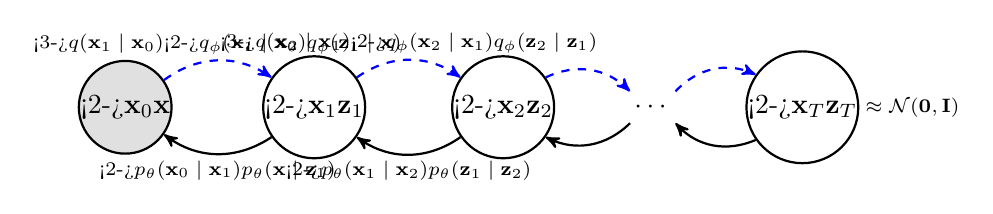
\begin{tikzpicture}
  \node[gm obs]    (x)  at (0,0)   {\alt<2->{$\bx_0$}{$\bx$}};
  \node[gm latent] (z1) at (2.4,0) {\alt<2->{$\bx_1$}{$\bz_1$}};
  \node[gm latent] (z2) at (4.8,0) {\alt<2->{$\bx_2$}{$\bz_2$}};
  \node            (zd) at (6.7,0) {$\cdots$};
  \node[gm latent] (zT) at (8.6,0) {\alt<2->{$\bx_T$}{$\bz_T$}};
 
  % encoder (inference), drawn above
  \draw[gm inf] (x)  to[bend left=35] node[gm lab, above] {\alt<3->{$q(\bx_1 \mid \bx_0)$}{\alt<2->{$q_\phi(\bx_1 \mid \bx_0)$}{$q_\phi(\bz_1 \mid \bx)$}}} (z1);
  \draw[gm inf] (z1) to[bend left=35] node[gm lab, above] {\alt<3->{$q(\bx_2 \mid \bx_1)$}{\alt<2->{$q_\phi(\bx_2 \mid \bx_1)$}{$q_\phi(\bz_2 \mid \bz_1)$}}} (z2);
  \draw[gm inf] (z2) to[bend left=35] (zd);
  \draw[gm inf] (zd) to[bend left=35] (zT);
 
  % decoder (generation), drawn below
  \draw[gm gen] (z1) to[bend left=35] node[gm lab, below] {\alt<2->{$p_\theta(\bx_0 \mid \bx_1)$}{$p_\theta(\bx \mid \bz_1)$}} (x);
  \draw[gm gen] (z2) to[bend left=35] node[gm lab, below] {\alt<2->{$p_\theta(\bx_1 \mid \bx_2)$}{$p_\theta(\bz_1 \mid \bz_2)$}} (z1);
  \draw[gm gen] (zd) to[bend left=35] (z2);
  \draw[gm gen] (zT) to[bend left=35] (zd);
 
  % restriction 3: known final distribution
  \node[gm lab, anchor=west, visible on=<4->] at (zT.east) {$\approx \mathcal{N}(\mathbf{0}, \mathbf{I})$};
\end{tikzpicture}
 
\vfill
 
\end{frame}




\begin{frame}{Diffusion Models: Intuition}
 
\vfill
 
\begin{itemize}
\item Idea: gradually turn data into noise, and learn to reverse this process \citebutton{Ho et al.\ (2020)\cite{ho2020denoising}}{https://arxiv.org/abs/2006.11239}
\item \textbf{Forward process} $q$: fixed, adds a little noise in each step
\item \textbf{Reverse process} $p_\theta$: learned, removes a little noise in each step
\end{itemize}
 
\vfill
 
\begin{center}
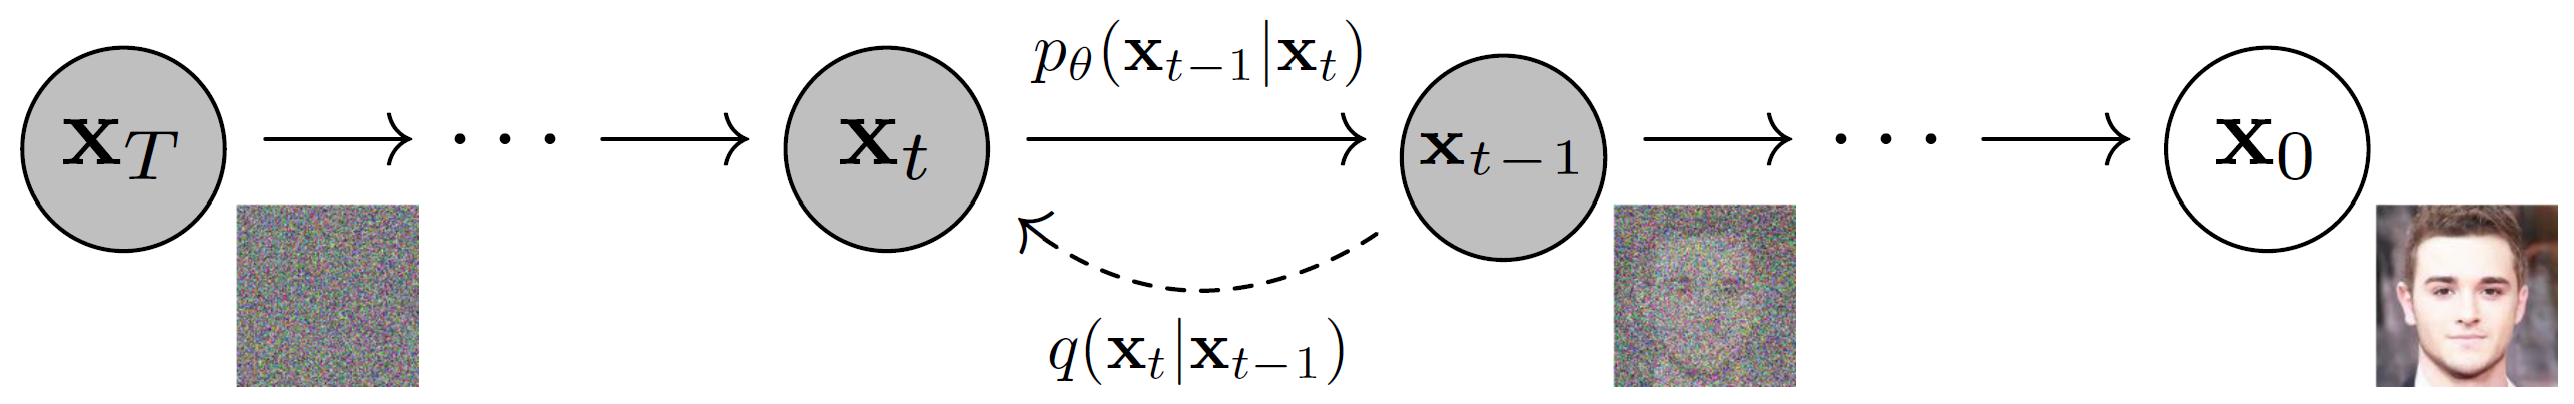
\includegraphics[width=\textwidth]{figure/diffusion_intuition.png}
\end{center}
 
\vfill
 
\end{frame}
 
 
 
 \begin{frame}{Forward Process}
 
\vfill
 
\begin{itemize}
\item The encoder is a fixed Markov chain without learnable parameters:
\begin{equation*}
q(\bx_{1:T} \mid \bx_0) = \prod_{t=1}^{T} q(\bx_t \mid \bx_{t-1})
\end{equation*}
\item We start with a sample $\bx_0$ and add Gaussian noise at each step:
\begin{equation*}
q(\bx_t \mid \bx_{t-1}) = \mathcal{N}\big(\bx_t; \sqrt{\alpha_t}\, \bx_{t-1}, (1 - \alpha_t)\, \mathbf{I}\big)
\end{equation*}
\item Equivalently: $\bx_t = \sqrt{\alpha_t}\, \bx_{t-1} + \sqrt{1 - \alpha_t}\, \boldsymbol{\epsilon}_t$ with $\boldsymbol{\epsilon}_t \sim \mathcal{N}(\mathbf{0}, \mathbf{I})$
\item \textbf{Noise schedule} $\alpha_1, \dots, \alpha_T \in (0, 1)$: hyperparameters
\end{itemize}

\vfill

\begin{center}
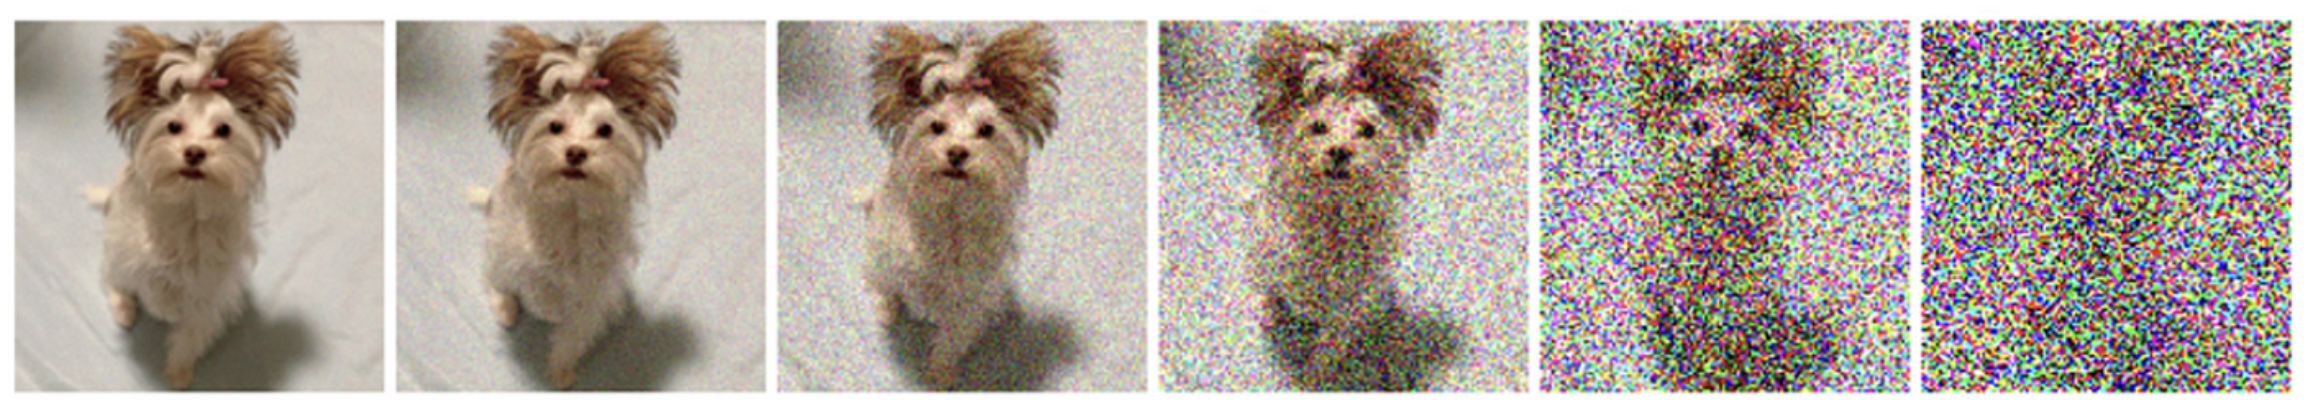
\includegraphics[width=\textwidth]{figure/noising.png}
\end{center}
 
\vfill
 
\end{frame}



\begin{frame}{Closed-Form Marginals}
 
\vfill
 
\begin{itemize}
\item Unrolling the recursion:
\begin{align*}
\bx_t &= \sqrt{\alpha_t}\, \bx_{t-1} + \sqrt{1 - \alpha_t}\, \boldsymbol{\epsilon}_t\\
&= \sqrt{\alpha_t} \, \big( \sqrt{\alpha_{t-1}}\, \bx_{t-2} + \sqrt{1 - \alpha_{t-1}}  \, \boldsymbol{\epsilon}_{t-1}\big)  + \sqrt{1 - \alpha_t}\, \boldsymbol{\epsilon}_t\\
&= \sqrt{\alpha_t \alpha_{t-1}}\, \bx_{t-2} + \sqrt{\alpha_t (1 - \alpha_{t-1})}\, \boldsymbol{\epsilon}_{t-1} + \sqrt{1 - \alpha_t}\, \boldsymbol{\epsilon}_t\\
&= \sqrt{\alpha_t \alpha_{t-1}}\, \bx_{t-2} + \sqrt{1 - \alpha_t \alpha_{t-1}}\, \boldsymbol{\epsilon}, \qquad \boldsymbol{\epsilon} \sim \mathcal{N}(\mathbf{0}, \mathbf{I})\\
&= \dots = \sqrt{\bar{\alpha}_t}\, \bx_0 + \sqrt{1 - \bar{\alpha}_t}\, \boldsymbol{\epsilon}, \qquad \bar{\alpha}_t := \prod_{s=1}^{t} \alpha_s
\end{align*}
\item \vspace{-5pt}Hence $q(\bx_t \mid \bx_0) = \mathcal{N}\big(\bx_t; \sqrt{\bar{\alpha}_t}\, \bx_0, (1 - \bar{\alpha}_t)\, \mathbf{I}\big)$
\item We can jump to any $t$ directly, without simulating the chain
\item $\bar{\alpha}_t$ decreases from $\approx 1$ to $\approx 0$, so $q(\bx_T \mid \bx_0) \approx \mathcal{N}(\mathbf{0}, \mathbf{I})$: $\bx_T$ carries (almost) no information about $\bx_0$
\end{itemize}
 
\vfill
 
\end{frame}




\begin{frame}{Backward Process}
 
\vfill
 
\begin{itemize}
\item Generative model (decoder):
\begin{equation*}
p_\theta(\bx_{0:T}) = p(\bx_T) \prod_{t=1}^{T} p_\theta(\bx_{t-1} \mid \bx_t), \qquad p(\bx_T) = \mathcal{N}(\mathbf{0}, \mathbf{I})
\end{equation*}
\item We do not know this process, but we will try to learn it from data
\item Each step is Gaussian (mean predicted by a neural network):
\begin{equation*}
p_\theta(\bx_{t-1} \mid \bx_t) = \mathcal{N}\big(\bx_{t-1}; \boldsymbol{\mu}_\theta(\bx_t, t), \sigma_t^2\, \mathbf{I}\big)
\end{equation*}
\item To generate from this model, we sample $\bx_T \sim \mathcal{N}(\mathbf{0}, \mathbf{I})$, then sample $\bx_{t-1} \sim p_\theta(\bx_{t-1} \mid \bx_t)$ for $t = T, \dots, 1$
\item The ideal reverse step $q(\bx_{t-1} \mid \bx_t)$ is intractable but approximately Gaussian for small noise steps
\end{itemize}
 
\vfill
 
\end{frame}
 
 
 
 \begin{frame}{Diffusion Model Training Intuition}
 
 \vfill
 
 
 \begin{itemize}
 \item Our goal is to learn the backward process $p_\theta(\bx_{t-1} \mid \bx_t)$ from the forward process $q(\bx_{t} \mid \bx_{t-1})$
 \item We will use the KL divergence for that
 \end{itemize}
 
 \vfill

\begin{center}
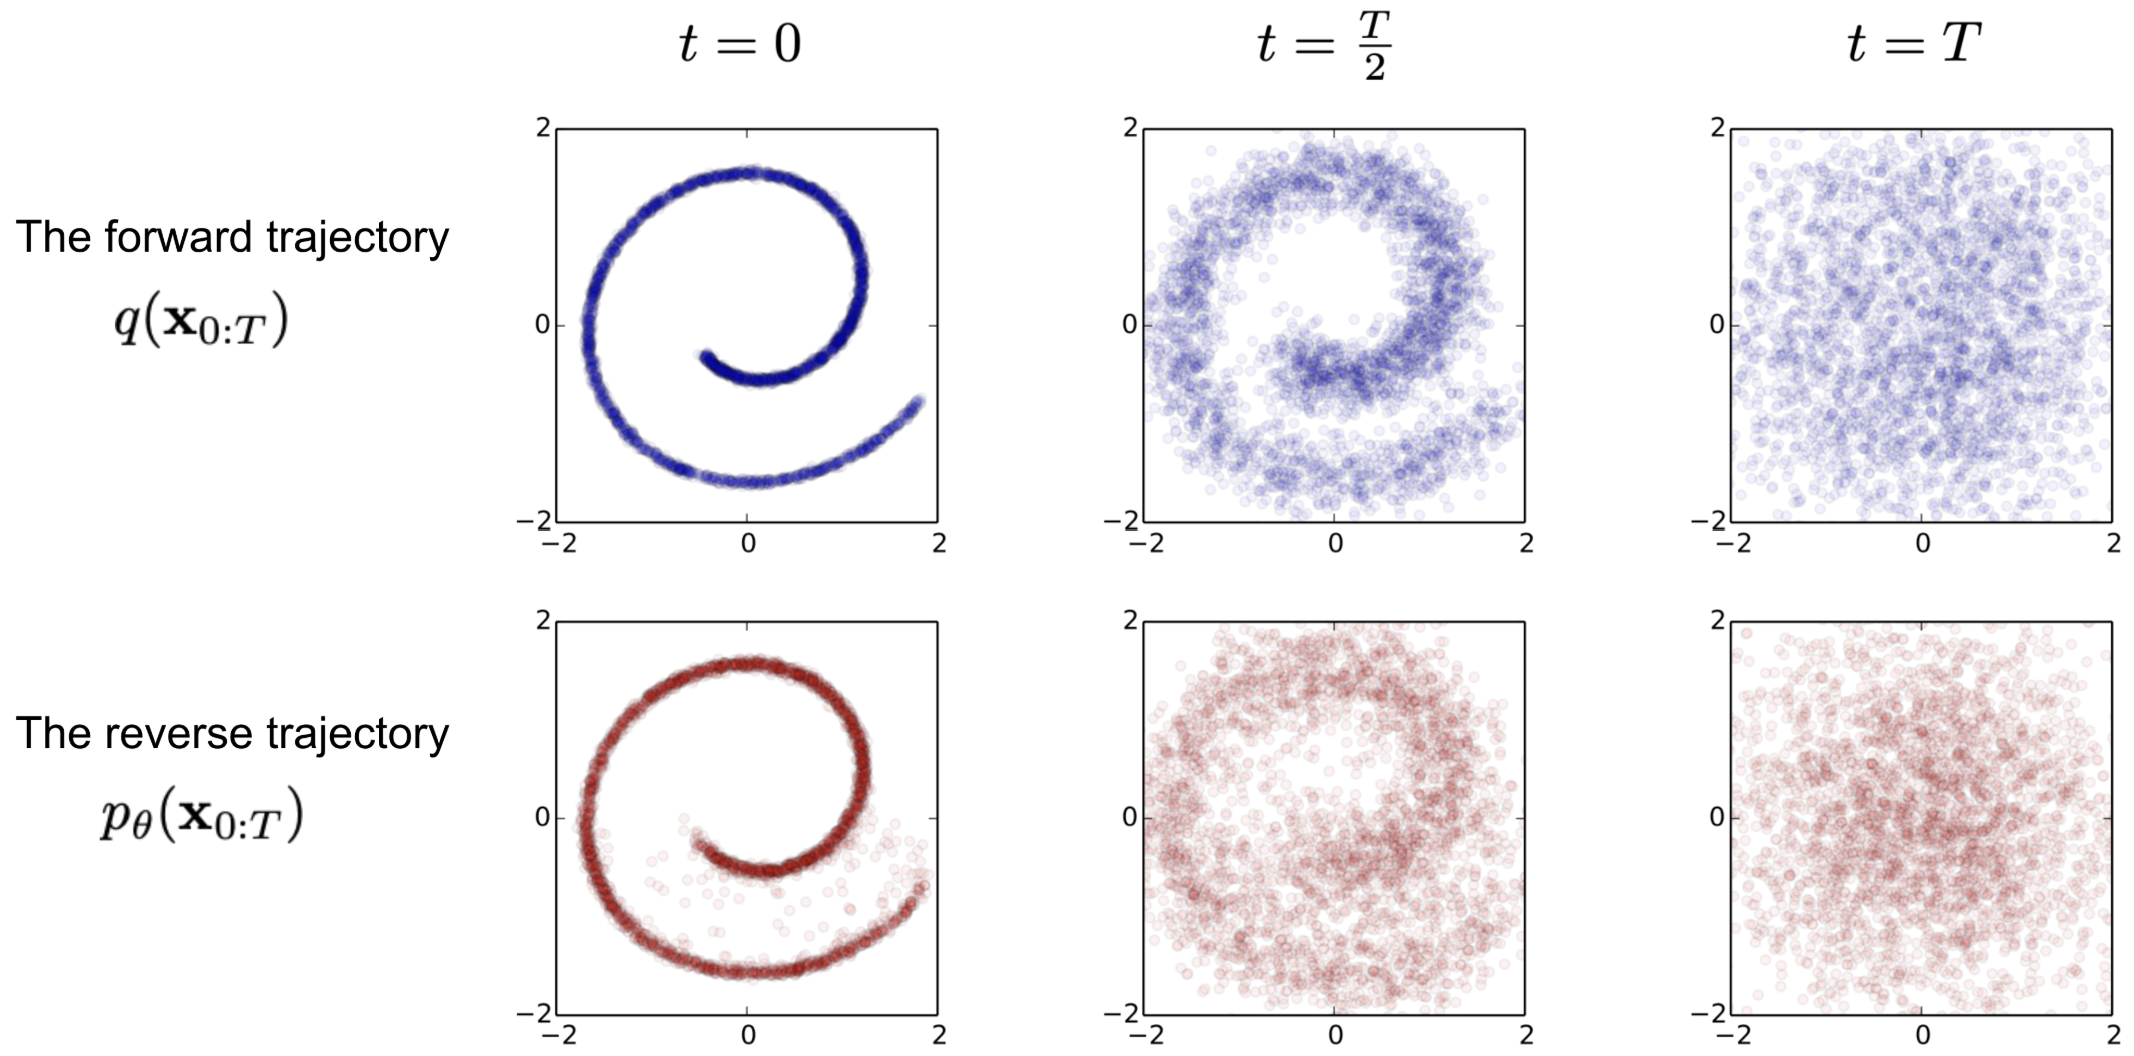
\includegraphics[width=0.9\textwidth]{figure/forward_backward.png}
\end{center}

\vfill
 \end{frame}
 
 
 
 
 
\begin{frame}{ELBO for Diffusion Models (I)}

\vfill

\begin{itemize}
\item Markovian HVAE ELBO with $\bz_t = \bx_t$ and a fixed encoder, so it only depends on $\theta$ ($\mathbb{E}_q$ short for $\mathbb{E}_{q(\bx_{1:T} \mid \bx_0)}$):
\begin{equation*}
\operatorname{ELBO}(\theta; \bx_0) = \mathbb{E}_{q}\left[\log \frac{p(\bx_T)\, p_\theta(\bx_0 \mid \bx_1) \prod_{t=2}^{T} p_\theta(\bx_{t-1} \mid \bx_t)}{q(\bx_1 \mid \bx_0) \prod_{t=2}^{T} q(\bx_t \mid \bx_{t-1})}\right]
\end{equation*}
\item Key trick: rewrite the encoder steps using $\bx_0$ since $q(\bx_{t-1} \mid \bx_t)$ is intractable, but $q(\bx_{t-1} \mid \bx_t, \bx_0)$ is not!
\end{itemize}

\vfill

\end{frame}


\begin{frame}{ELBO for Diffusion Models (II)}

\vfill

\begin{itemize}
\item Apply Markov property, then Bayes' rule (conditioned on $\bx_0$):
\begin{equation*}
q(\bx_t \mid \bx_{t-1}) = q(\bx_t \mid \bx_{t-1}, \bx_0) = \frac{q(\bx_{t-1} \mid \bx_t, \bx_0)\, q(\bx_t \mid \bx_0)}{q(\bx_{t-1} \mid \bx_0)}
\end{equation*}
\item The product of ratios $\prod_{t=2}^{T} \frac{q(\bx_t \mid \bx_0)}{q(\bx_{t-1} \mid \bx_0)}$ telescopes:
\begin{equation*}
\frac{q(\bx_2 \mid \bx_0)}{q(\bx_1 \mid \bx_0)} \cdot \frac{q(\bx_3 \mid \bx_0)}{q(\bx_2 \mid \bx_0)} \cdots \frac{q(\bx_T \mid \bx_0)}{q(\bx_{T-1} \mid \bx_0)} = \frac{q(\bx_T \mid \bx_0)}{q(\bx_1 \mid \bx_0)}
\end{equation*}
\item Hence the denominator of the ELBO becomes:
\begin{equation*}
q(\bx_1 \mid \bx_0) \prod_{t=2}^{T} q(\bx_t \mid \bx_{t-1}) = q(\bx_T \mid \bx_0) \prod_{t=2}^{T} q(\bx_{t-1} \mid \bx_t, \bx_0)
\end{equation*}
\item Interpretation: $q(\bx_{1:T} \mid \bx_0)$ factorized in reverse order
\end{itemize}

\vfill

\end{frame}


\begin{frame}{ELBO for Diffusion Models (III)}

\vfill

\begin{itemize}
\item Substituting the reverse factorization and splitting the logarithm:
{\small
\begin{align*}
\operatorname{ELBO}  &= \mathbb{E}_{q}\left[\log \frac{p(\bx_T)\, p_\theta(\bx_0 \mid \bx_1) \prod_{t=2}^{T} p_\theta(\bx_{t-1} \mid \bx_t)}{q(\bx_T \mid \bx_0) \prod_{t=2}^{T} q(\bx_{t-1} \mid \bx_t, \bx_0)}\right]\\[-0.5ex]
&= \mathbb{E}_{q}\bigg[\log p_\theta(\bx_0 \mid \bx_1) + \log \frac{p(\bx_T)}{q(\bx_T \mid \bx_0)} + \sum_{t=2}^{T} \log \frac{p_\theta(\bx_{t-1} \mid \bx_t)}{q(\bx_{t-1} \mid \bx_t, \bx_0)}\bigg]\\
&= \underbrace{\mathbb{E}_{q(\bx_1 \mid \bx_0)}\big[\log p_\theta(\bx_0 \mid \bx_1)\big]}_{\text{reconstruction term}} - \underbrace{\operatorname{KL}\big(q(\bx_T \mid \bx_0) \,\|\, p(\bx_T)\big)}_{\text{prior matching term}}\\[-1ex]
&\quad - \sum_{t=2}^{T} \underbrace{\mathbb{E}_{q(\bx_t \mid \bx_0)}\Big[\operatorname{KL}\big(q(\bx_{t-1} \mid \bx_t, \bx_0) \,\|\, p_\theta(\bx_{t-1} \mid \bx_t)\big)\Big]}_{\text{denoising matching term}}
\end{align*}
}
\item NB: expectations reduce to the latents each term involves
\end{itemize}

\vfill

\end{frame}



\begin{frame}{ELBO Interpretation}
 
\vfill

 
\begin{itemize}
\item \textbf{Reconstruction term}: recover $\bx_0$ from the slightly noisy $\bx_1$
\item \textbf{Prior matching term}: no learnable parameters and $\approx 0$ (why?)
\item \textbf{Denoising matching term}: each learned reverse step $p_\theta(\bx_{t-1} \mid \bx_t)$ should match the ``ground-truth'' reverse step $q(\bx_{t-1} \mid \bx_t, \bx_0)$, which knows $\bx_0$
\item The derivation only used the Markov property and Bayes' rule, so it holds for \emph{any} forward process
\end{itemize}
 
\vfill
 
\end{frame}



\begin{frame}{Tractable Reverse Step}

\vfill

\begin{itemize}
\item Bayes' rule, where all three terms are Gaussians we know:
{\small
\begin{align*}
&q(\bx_{t-1} \mid \bx_t, \bx_0) = \frac{q(\bx_t \mid \bx_{t-1})\, q(\bx_{t-1} \mid \bx_0)}{q(\bx_t \mid \bx_0)}\\
&\quad = \frac{\mathcal{N}\big(\bx_t; \sqrt{\alpha_t}\, \bx_{t-1}, (1 - \alpha_t)\, \mathbf{I}\big)\, \mathcal{N}\big(\bx_{t-1}; \sqrt{\bar{\alpha}_{t-1}}\, \bx_0, (1 - \bar{\alpha}_{t-1})\, \mathbf{I}\big)}{\mathcal{N}\big(\bx_t; \sqrt{\bar{\alpha}_t}\, \bx_0, (1 - \bar{\alpha}_t)\, \mathbf{I}\big)}
\end{align*}
}
\item This can be rewritten as another Gaussian:
\begin{align*}
q(\bx_{t-1} \mid \bx_t, \bx_0) &= \mathcal{N}\big(\bx_{t-1}; \boldsymbol{\mu}_q(\bx_t, \bx_0), \sigma_q^2(t)\, \mathbf{I}\big)\\
\boldsymbol{\mu}_q(\bx_t, \bx_0) &= \frac{\sqrt{\alpha_t}\,(1 - \bar{\alpha}_{t-1})\, \bx_t + \sqrt{\bar{\alpha}_{t-1}}\,(1 - \alpha_t)\, \bx_0}{1 - \bar{\alpha}_t}\\
\sigma_q^2(t) &= \frac{(1 - \alpha_t)(1 - \bar{\alpha}_{t-1})}{1 - \bar{\alpha}_t}
\end{align*}
\end{itemize}

\vfill

\end{frame}



\begin{frame}{Reverse Step Intuition}

\vfill

\begin{center}
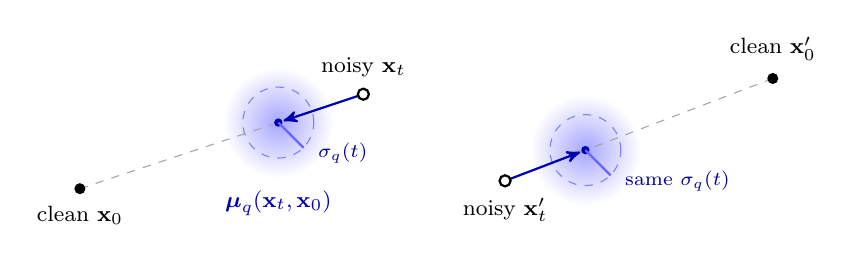
\begin{tikzpicture}
  % ---- first pair (x_0, x_t) ------------------------------------------------
  \coordinate (x0) at (0,0);
  \coordinate (xt) at (3.6,1.2);
  \coordinate (mu) at (2.52,0.84);
  \shade[inner color=blue!35, outer color=white] (mu) circle (0.7);
  \draw[blue!50, dashed] (mu) circle (0.45);
  \draw[black!35, dashed] (x0) -- (xt);
  \draw[->, thick, blue!70!black, shorten >=2pt] (xt) -- (mu);
  \fill (x0) circle (2pt);
  \node[font=\footnotesize, anchor=north] at (0,-0.1) {clean $\bx_0$};
  \draw[thick, fill=white] (xt) circle (2pt);
  \node[font=\footnotesize, anchor=south] at (3.6,1.3) {noisy $\bx_t$};
  \fill[blue!70!black] (mu) circle (1.5pt);
  \node[font=\footnotesize, text=blue!70!black, anchor=north] at (2.52,0.1) {$\boldsymbol{\mu}_q(\bx_t, \bx_0)$};
  \draw[blue!60, thick] (mu) -- (2.84,0.52);
  \node[font=\scriptsize, text=blue!60!black, anchor=west] at (2.9,0.45) {$\sigma_q(t)$};

  % ---- second pair (x_0', x_t'), same t --------------------------------------
  \begin{scope}
    \coordinate (y0) at (8.8,1.4);
    \coordinate (yt) at (5.4,0.1);
    \coordinate (nu) at (6.42,0.49);
    \shade[inner color=blue!35, outer color=white] (nu) circle (0.7);
    \draw[blue!50, dashed] (nu) circle (0.45);
    \draw[black!35, dashed] (y0) -- (yt);
    \draw[->, thick, blue!70!black, shorten >=2pt] (yt) -- (nu);
    \fill (y0) circle (2pt);
    \node[font=\footnotesize, anchor=south] at (8.8,1.5) {clean $\bx_0'$};
    \draw[thick, fill=white] (yt) circle (2pt);
    \node[font=\footnotesize, anchor=north] at (5.4,0.0) {noisy $\bx_t'$};
    \fill[blue!70!black] (nu) circle (1.5pt);
    \draw[blue!60, thick] (nu) -- (6.74,0.17);
    \node[font=\scriptsize, text=blue!60!black, anchor=west] at (6.8,0.1) {same $\sigma_q(t)$};
  \end{scope}
\end{tikzpicture}
\end{center}

\vfill

\begin{itemize}
\item Mean: $\boldsymbol{\mu}_q(\bx_t, \bx_0) = c_t\, \bx_t + c_0\, \bx_0$ with $c_t + c_0 \approx 1$, i.e., a step from the noisy $\bx_t$ toward the clean $\bx_0$ (small, except close to $t = 1$)
\item Variance: $\sigma_q^2(t)$ only depends on the noise schedule, so all pairs $(\bx_0, \bx_t)$ at step $t$ get the same spread
\end{itemize}

\vfill

\end{frame}


\begin{frame}{How the Reverse Step Changes over Time}
 
\vfill
 
\begin{center}
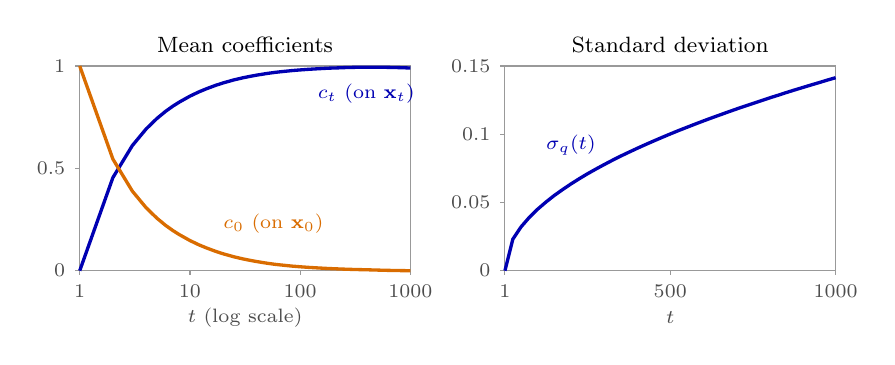
\begin{tikzpicture}[font=\scriptsize]
  % ======== left panel: mean coefficients (log t axis) ========
  \begin{scope}
    \draw[black!40] (0,0) rectangle (4.2,2.6);
    \foreach \x/\lab in {0/1, 1.4/10, 2.8/100, 4.2/1000} {
      \draw[black!40] (\x,0) -- (\x,-0.06) node[below, text=black!70] {\lab};
    }
    \foreach \y/\lab in {0/0, 1.3/0.5, 2.6/1} {
      \draw[black!40] (0,\y) -- (-0.06,\y) node[left, text=black!70] {\lab};
    }
    \node[text=black!70] at (2.1,-0.6) {$t$ (log scale)};
    \node[font=\footnotesize, anchor=south] at (2.1,2.65) {Mean coefficients};
    \draw[very thick, blue!70!black] plot coordinates {(0.000,0.000) (0.421,1.182) (0.668,1.589) (0.843,1.800) (0.979,1.932) (1.089,2.023) (1.183,2.090) (1.264,2.141) (1.400,2.217) (1.511,2.270) (1.605,2.309) (1.723,2.353) (1.821,2.385) (1.957,2.423) (2.068,2.449) (2.162,2.468) (2.243,2.483) (2.379,2.505) (2.489,2.520) (2.583,2.530) (2.701,2.542) (2.800,2.550) (2.911,2.558) (3.047,2.566) (3.157,2.572) (3.279,2.576) (3.381,2.580) (3.507,2.583) (3.643,2.584) (3.779,2.585) (3.889,2.583) (3.983,2.581) (4.101,2.578) (4.200,2.574)};
    \draw[very thick, orange!85!black] plot coordinates {(0.000,2.600) (0.421,1.418) (0.668,1.011) (0.843,0.800) (0.979,0.668) (1.089,0.577) (1.183,0.510) (1.264,0.459) (1.400,0.383) (1.511,0.330) (1.605,0.291) (1.723,0.247) (1.821,0.215) (1.957,0.177) (2.068,0.151) (2.162,0.132) (2.243,0.117) (2.379,0.095) (2.489,0.080) (2.583,0.070) (2.701,0.058) (2.800,0.050) (2.911,0.042) (3.047,0.034) (3.157,0.028) (3.279,0.023) (3.381,0.019) (3.507,0.015) (3.643,0.012) (3.779,0.008) (3.889,0.005) (3.983,0.003) (4.101,0.001) (4.200,0.000)};
    \node[text=blue!70!black, anchor=south west] at (2.9,2.0) {$c_t$ (on $\bx_t$)};
    \node[text=orange!85!black, anchor=south west] at (1.7,0.35) {$c_0$ (on $\bx_0$)};
  \end{scope}
 
  % ======== right panel: standard deviation (linear t axis) ========
  \begin{scope}[xshift=5.4cm]
    \draw[black!40] (0,0) rectangle (4.2,2.6);
    \foreach \x/\lab in {0/1, 2.1/500, 4.2/1000} {
      \draw[black!40] (\x,0) -- (\x,-0.06) node[below, text=black!70] {\lab};
    }
    \foreach \y/\lab in {0/0, 0.867/0.05, 1.733/0.1, 2.6/0.15} {
      \draw[black!40] (0,\y) -- (-0.06,\y) node[left, text=black!70] {\lab};
    }
    \node[text=black!70] at (2.1,-0.6) {$t$};
    \node[font=\footnotesize, anchor=south] at (2.1,2.65) {Standard deviation};
    \draw[very thick, blue!70!black] plot coordinates {(0.000,0.000) (0.101,0.402) (0.206,0.558) (0.311,0.679) (0.416,0.782) (0.521,0.872) (0.626,0.955) (0.732,1.030) (0.837,1.101) (0.942,1.167) (1.047,1.230) (1.152,1.289) (1.257,1.346) (1.362,1.401) (1.467,1.454) (1.572,1.504) (1.677,1.553) (1.783,1.601) (1.888,1.647) (1.993,1.692) (2.098,1.736) (2.203,1.779) (2.308,1.820) (2.413,1.861) (2.518,1.901) (2.623,1.940) (2.729,1.978) (2.834,2.016) (2.939,2.053) (3.044,2.089) (3.149,2.124) (3.254,2.159) (3.359,2.194) (3.464,2.227) (3.569,2.261) (3.674,2.294) (3.780,2.326) (3.885,2.358) (3.990,2.389) (4.095,2.421) (4.200,2.451)};
    \node[text=blue!70!black, anchor=west] at (0.4,1.6) {$\sigma_q(t)$};
  \end{scope}
\end{tikzpicture}
 
\end{center}
  
\begin{itemize}
\item DDPM \citebutton{Ho et al.\ (2020)\cite{ho2020denoising}}{https://arxiv.org/abs/2006.11239}: $T = 1000$, $1 - \alpha_t$ from $10^{-4}$ to $0.02$
\item $c_t \approx 1$ for almost all $t$: each reverse step stays close to $\bx_t$
\item $c_0$ is only large near $t = 1$ (where $\boldsymbol{\mu}_q = \bx_0$) and gives a small nudge toward $\bx_0$ elsehere
\item $\sigma_q(t)$ grows with $t$
\end{itemize}
 
\vfill
 
\end{frame}
 
 
 
 \begin{frame}{Interim Recap}


\vfill

\begin{itemize}
\item We model reverse steps as Gaussians:
\begin{equation*}
p_\theta(\bx_{t-1} \mid \bx_t) = \mathcal{N}\big(\bx_{t-1}; \boldsymbol{\mu}_\theta(\bx_t, t), \sigma_t^2\, \mathbf{I}\big)
\end{equation*}
\item We want each learned reverse step $p_\theta(\bx_{t-1} \mid \bx_t)$ to match the ``ground-truth'' reverse step $q(\bx_{t-1} \mid \bx_t, \bx_0)$
\item We now have an exact formula for the ``ground-truth'' reverse step:
\begin{equation*}
q(\bx_{t-1} \mid \bx_t, \bx_0) = \mathcal{N}\big(\bx_{t-1}; \boldsymbol{\mu}_q(\bx_t,\bx_0), \sigma_q^2(t)\, \mathbf{I}\big)
\end{equation*}
\item So why not simply set $p_\theta(\bx_{t-1} \mid \bx_t) := q(\bx_{t-1} \mid \bx_t, \bx_0)$?
\item<2-> The variance is easy: $\sigma_t^2 := \sigma_q^2(t)$
\item<2-> The mean is the problem: $\boldsymbol{\mu}_q$ needs $\bx_0$, but $p_\theta$ only sees $\bx_t$
\end{itemize}

\vfill

\end{frame}


\begin{frame}{Learning to Recover the Original Data}

\vfill

\begin{itemize}
\item Solution: we plug in a neural network prediction $\hat{\bx}_\theta(\bx_t, t) \approx \bx_0$:
\begin{equation*}
p_\theta(\bx_{t-1} \mid \bx_t) = \mathcal{N}\big(\bx_{t-1}; \boldsymbol{\mu}_q(\bx_t, \hat{\bx}_\theta(\bx_t, t)), \sigma_q^2(t)\, \mathbf{I}\big)
\end{equation*}
\item KL between Gaussians with equal covariance:
\begin{align*}
&\operatorname{KL}\big(q(\bx_{t-1} \mid \bx_t, \bx_0) \,\|\, p_\theta(\bx_{t-1} \mid \bx_t)\big)\\
&\quad = \frac{1}{2\sigma_q^2(t)} \big\| \boldsymbol{\mu}_q(\bx_t, \bx_0) - \boldsymbol{\mu}_q(\bx_t, \hat{\bx}_\theta(\bx_t, t)) \big\|^2\\
&\quad = \underbrace{\frac{c_0^2}{2\sigma_q^2(t)}}_{=:\, w_t} \big\| \hat{\bx}_\theta(\bx_t, t) - \bx_0 \big\|^2
\end{align*}
\item $w_t$ is large at low noise (large $c_0$) and tiny at high noise
\item \textbf{A diffusion model is a denoiser that learns to recover the original data at all noise levels!}
\end{itemize}

\vfill

\end{frame}
 
 



\begin{frame}{Training}

\vfill

\begin{itemize}
\item Objective (the prior matching term is constant):
\begin{equation*}
\min_\theta \sum_{t=2}^{T} \mathbb{E}_{q(\bx_t \mid \bx_0)}\Big[w_t\, \big\| \hat{\bx}_\theta(\bx_t, t) - \bx_0 \big\|^2\Big]
\end{equation*}
\item Since $w_t$ is largest for small $t$, the loss implicitly focuses low-noise reconstructions
\item The reconstruction term ($t = 1$) can be handled analogously
\item Repeat until convergence (Monte Carlo estimate):
\begin{enumerate}
\item Sample a training example $\bx_0$
\item Sample a noise level $t \sim \mathcal{U}\{2, \dots, T\}$
\item Sample $\boldsymbol{\epsilon} \sim \mathcal{N}(\mathbf{0}, \mathbf{I})$ and set $\bx_t = \sqrt{\bar{\alpha}_t}\, \bx_0 + \sqrt{1 - \bar{\alpha}_t}\, \boldsymbol{\epsilon}$
\item Take a gradient step on $w_t\, \| \hat{\bx}_\theta(\bx_t, t) - \bx_0 \|^2$
\end{enumerate}
\item One network $\hat{\bx}_\theta$ is shared across all noise levels
\end{itemize}

\vfill

\end{frame}



\begin{frame}{Diffusion Models in Action}

\vfill

\begin{center}
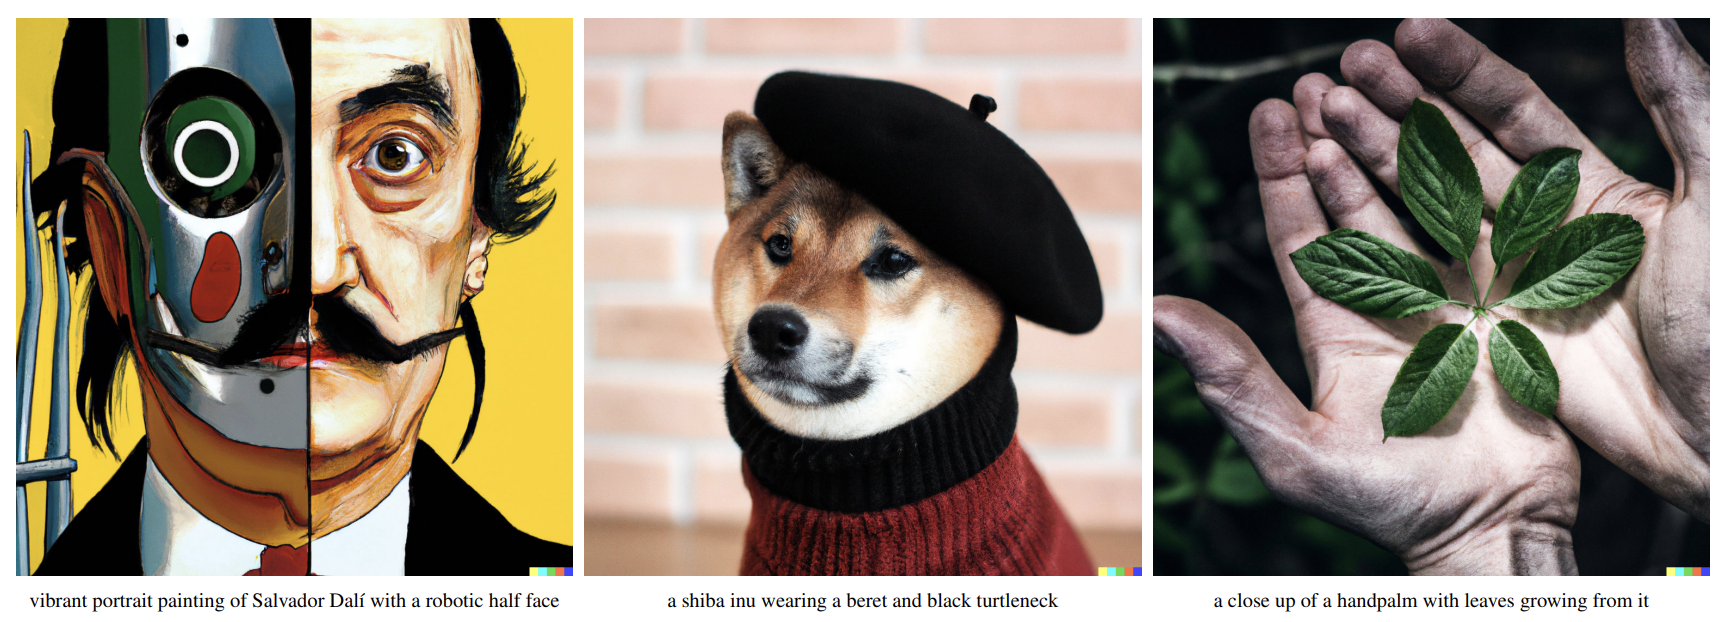
\includegraphics[width=\linewidth]{figure/dalle.png}
\end{center}

\vfill

\begin{itemize}
\item Diffusion models power most image generators (e.g., DALLE)
\item But images are continuous, while text is discrete: how do we add ``noise'' to text?
\end{itemize}

\vfill

\end{frame}

 
 

\section{Masked Diffusion LLMs}

 
\begin{frame}{Why Diffusion for Text?}

\def\cmark{\textcolor{green!50!black}{\checkmark}}
\def\xmark{\textcolor{red!70!black}{$\times$}}

\vfill

\begin{center}
\renewcommand{\arraystretch}{1.5}
\begin{tabular}{>{\raggedright\arraybackslash}p{4.9cm} >{\raggedright\arraybackslash}p{4.9cm}}
\textbf{Autoregression} & \textbf{Diffusion} \\
\hline
\xmark\ Sequential generation & \cmark\ Parallel (fast) generation \\
\xmark\ Fixed number of steps & \cmark\ Flexible number of steps \\
\xmark\ Left-to-right context & \cmark\ Bidirectional context
\end{tabular}
\end{center}

\vfill


\centering
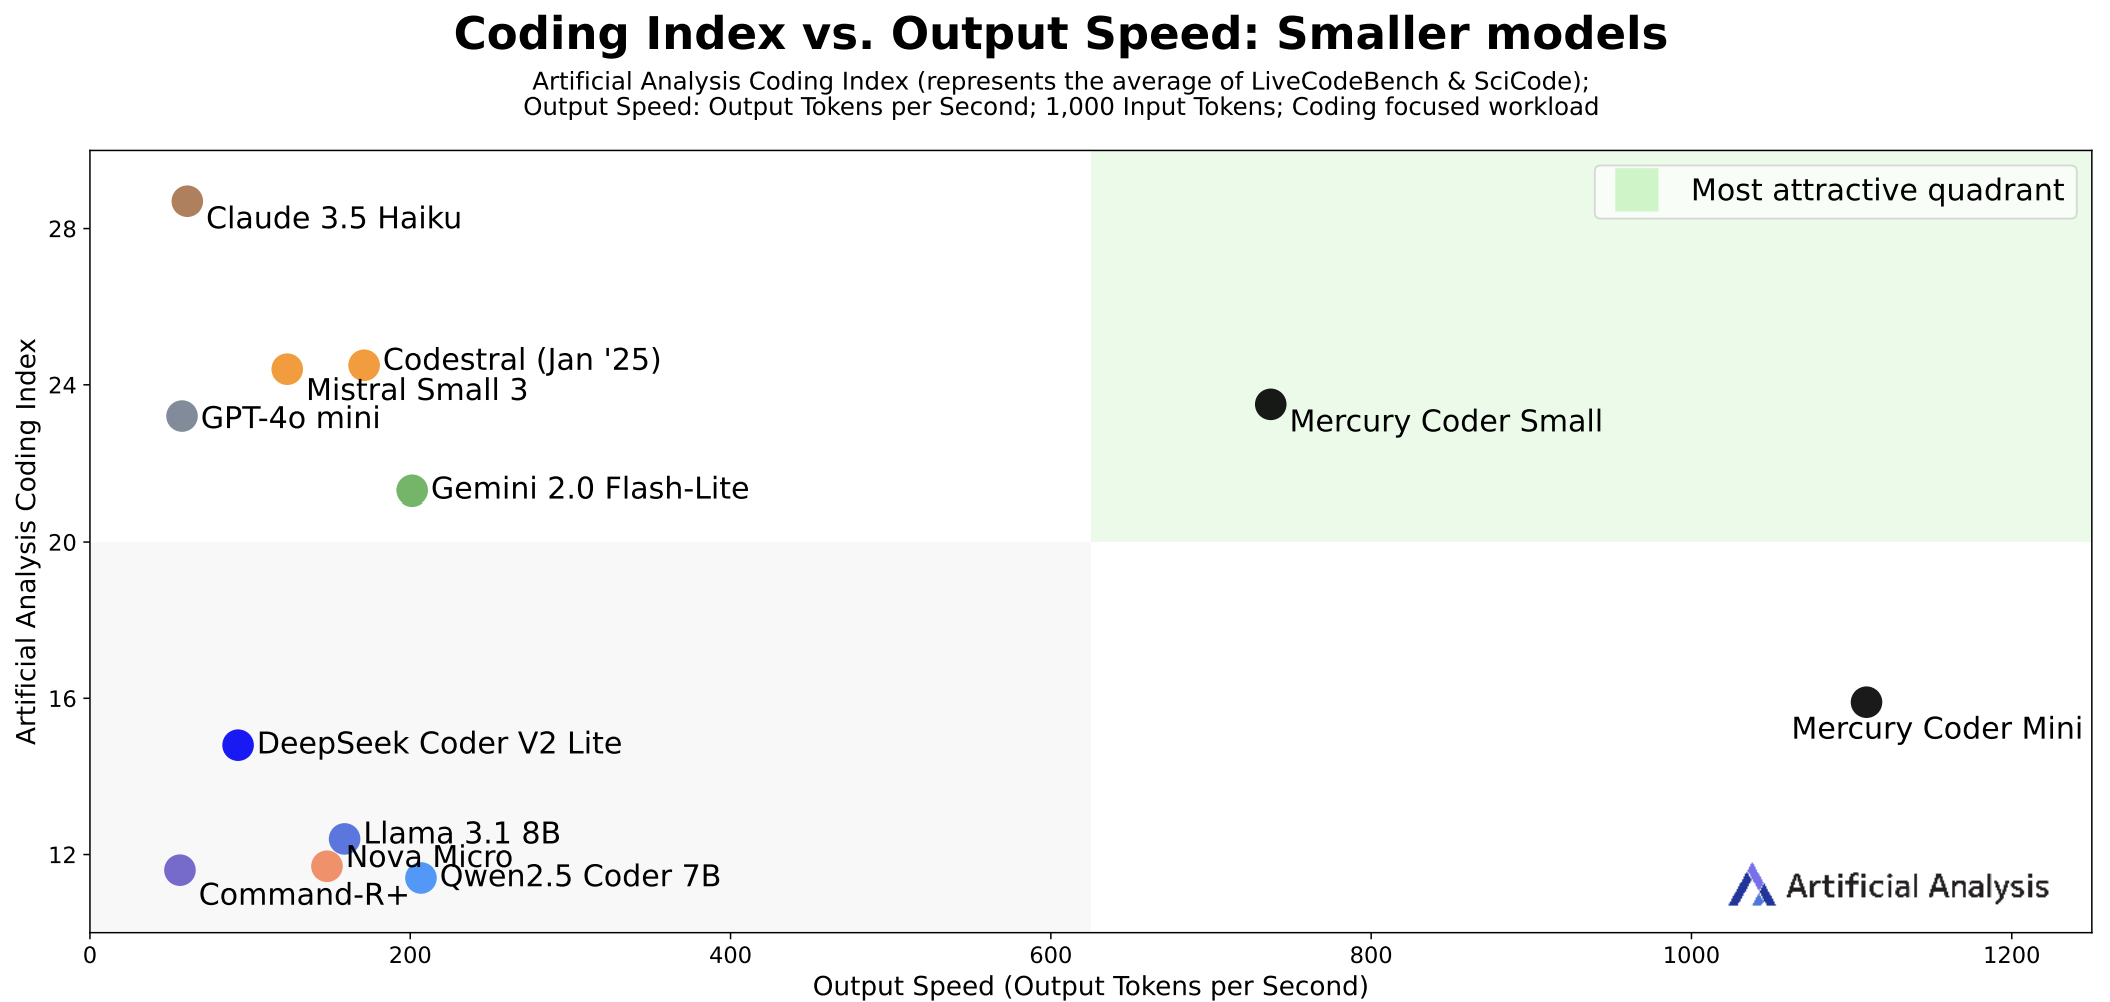
\includegraphics[width=0.8\linewidth]{figure/mercury_speed.png}

\vfill

\end{frame}



\begin{frame}{Masking as the Forward Process}
 
\vfill
 
\begin{itemize}
\item Tokens are one-hot vectors over $\vocab \cup \{\texttt{[MASK]}\}$
\item We start with a clean sequence $\bx_0 = (\bx_0^1, \dots, \bx_0^L)$
\item Tokens are masked independently ($\mathbf{m}$ denotes vector of \texttt{[MASK]}):
\begin{equation*}
q(\bx_t^\ell \mid \bx_0^\ell) = \operatorname{Cat}\big(\bx_t^\ell;\ \bar{\alpha}_t\, \bx_0^\ell + (1 - \bar{\alpha}_t)\, \mathbf{m}\big)
\end{equation*}
\item Keep the token with probability $\bar{\alpha}_t$, otherwise mask it
\item Masked tokens stay masked (\textbf{absorbing state})
\item $\bar{\alpha}_0 = 1$ and $\bar{\alpha}_T = 0$, so $\bx_T$ is all \texttt{[MASK]}
\end{itemize}
 
\vfill
 
\begin{center}
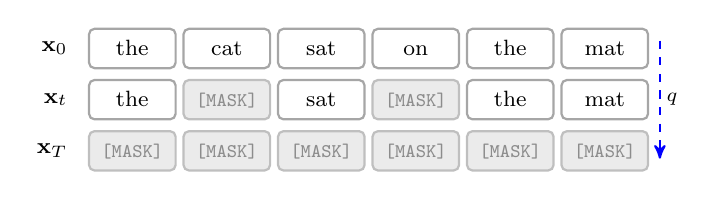
\begin{tikzpicture}[
  tok/.style={rounded corners=2pt, minimum width=1.1cm, minimum height=0.5cm, text height=1.6ex, text depth=0.4ex, inner sep=1pt, thick, font=\footnotesize, fill=white, draw=black!35},
  msk/.style={tok, fill=black!8, draw=black!25, text=black!45, font=\scriptsize\ttfamily},
]
  \foreach \w/\a/\b [count=\i from 0] in {the/0/1, cat/1/1, sat/0/1, on/1/1, the/0/1, mat/0/1} {
    \node[tok] at (\i*1.2, 0) {\w};
    \ifnum\a=1 \node[msk] at (\i*1.2, -0.65) {[MASK]}; \else \node[tok] at (\i*1.2, -0.65) {\w}; \fi
    \node[msk] at (\i*1.2, -1.3) {[MASK]};
  }
  \node[font=\footnotesize, anchor=east] at (-0.7, 0)    {$\bx_0$};
  \node[font=\footnotesize, anchor=east] at (-0.7, -0.65) {$\bx_t$};
  \node[font=\footnotesize, anchor=east] at (-0.7, -1.3)  {$\bx_T$};
  \draw[gm inf] (6.7, 0.1) -- (6.7, -1.4) node[gm lab, midway, right] {$q$};
\end{tikzpicture}
\end{center}
 
\vfill
 
\end{frame}
 
 

\begin{frame}{Tractable Reverse Step}
 
\vfill
 
\begin{itemize}
\item Unmasked tokens stay unmasked: if $\bx_t^\ell \neq \mathbf{m}$, then $\bx_{t-1}^\ell = \bx_t^\ell$
\item Masked tokens:
\begin{equation*}
q(\bx_{t-1}^\ell \mid \bx_t^\ell = \mathbf{m}, \bx_0^\ell) = \operatorname{Cat}\Big(\bx_{t-1}^\ell;\ w_t\, \bx_0^\ell + (1 - w_t)\, \mathbf{m}\Big)
\end{equation*}
\item A masked token is unmasked to $\bx_0^\ell$ with probability $w_t := \frac{\bar{\alpha}_{t-1} - \bar{\alpha}_t}{1 - \bar{\alpha}_t}$ and stays masked otherwise
\item Same structure as in the Gaussian case: a weighted combination of $\bx_t$ ($= \mathbf{m}$) and $\bx_0$
\end{itemize}
 
\vfill
 
\end{frame}



\begin{frame}{Learning to Recover the Original Tokens}
 
\vfill
 
\begin{itemize}
\item As before, $p_\theta(\bx_{t-1}^\ell \mid \bx_t)$ does not have access to $\bx_0$, so we predict it with a neural network, $\hat{\bx}_\theta^\ell(\bx_t)$, and compute:
\begin{equation*}
p_\theta(\bx_{t-1}^\ell \mid \bx_t) = \operatorname{Cat}\big(\bx_{t-1}^\ell;\ w_t\, \hat{\bx}_\theta^\ell(\bx_t) + (1 - w_t)\, \mathbf{m}\big) \quad \text{if } \bx_t^\ell = \mathbf{m}
\end{equation*}
\item Unmasked positions are copied, so their KL is $0$
\item Masked positions: KL simplifies as
\begin{equation*}
\operatorname{KL}\big(q(\bx_{t-1}^\ell \mid \bx_t^\ell, \bx_0^\ell) \,\|\, p_\theta(\bx_{t-1}^\ell \mid \bx_t)\big) = -\,w_t \log p_\theta(\bx_0^\ell \mid \bx_t)
\end{equation*}
\item $p_\theta(\bx_0^\ell \mid \bx_t)$ is the probability $\hat{\bx}_\theta^\ell(\bx_t)$ assigns to the correct token
\item Weighted cross-entropy (cf.\ $w_t \|\hat{\bx}_\theta - \bx_0\|^2$ in the Gaussian case)
\end{itemize}
 
\vfill
 
\end{frame}



\begin{frame}{Training Objective}
 
\vfill
 
\begin{itemize}
\item Prior matching term is $0$ (why?)
\item Negative ELBO \citebutton{Sahoo et al.\ (2024)\cite{sahoo2024simple}}{https://arxiv.org/abs/2406.07524}:
\begin{equation*}
\mathcal{L}(\theta) = \sum_{t=1}^{T} \mathbb{E}_{q(\bx_t \mid \bx_0)}\Big[w_t \sum_{\ell:\, \bx_t^\ell = \mathbf{m}} -\log p_\theta(\bx_0^\ell \mid \bx_t)\Big]
\end{equation*}
\item What has happened to the reconstruction term?
\item Linear schedule $\bar{\alpha}_t = 1 - t/T$: masking rate $r_t = t/T$ and $w_t = 1/t$, so
\begin{equation*}
\mathcal{L}(\theta) = \mathbb{E}_{t \sim \mathcal{U}\{1, \dots, T\}}\, \mathbb{E}_{q(\bx_t \mid \bx_0)}\Big[\frac{1}{r_t} \sum_{\ell:\, \bx_t^\ell = \mathbf{m}} -\log p_\theta(\bx_0^\ell \mid \bx_t)\Big]
\end{equation*}
\item Again, lightly masked inputs (low noise) get the largest weight
\end{itemize}
 
\vfill
 
\end{frame}



\begin{frame}{Surprise: MDLM Is (Almost) BERT!}
 
\colorlet{hl}{orange!85!black}
 
\vfill
 
\begin{itemize}
\item BERT: mask 15\% of the tokens and predict them \citebutton{Devlin et al.\ (2019)\cite{devlin-etal-2019-bert}}{https://aclanthology.org/N19-1423/}
\begin{equation*}
\mathcal{L}_{\text{BERT}}(\theta) = \mathbb{E}_{\bx_t:\ \text{15\% masked}}\Big[\sum_{\ell:\, \bx_t^\ell = \mathbf{m}} -\log p_\theta(\bx_0^\ell \mid \bx_t)\Big]
\end{equation*}
\item<2-> MDLM: same loss, with a \textcolor{hl}{random masking rate} and a \textcolor{hl}{weight}
\begin{equation*}
\mathcal{L}_{\text{MDLM}}(\theta) = \mathbb{E}_{\textcolor{hl}{r \sim \mathcal{U}(0, 1]}}\, \mathbb{E}_{\bx_t:\ r\ \text{masked}}\Big[\textcolor{hl}{\frac{1}{r}} \sum_{\ell:\, \bx_t^\ell = \mathbf{m}} -\log p_\theta(\bx_0^\ell \mid \bx_t)\Big]
\end{equation*}
\item<3-> These two changes turn the loss into an upper bound on $-\log p_\theta(\bx_0)$, making MDLMs  proper generative models
\item<3-> BERT never learns to predict from fully masked inputs, so it cannot generate from scratch
\end{itemize}
 
\vfill
 
\end{frame}
 
 
 
 \begin{frame}{Sampling}
 
\vfill
 
\begin{itemize}
\item Start from $\bx_T$: all \texttt{[MASK]} (output length fixed in advance)
\item For $t = T, \dots, 1$: predict $\hat{\bx}_\theta^\ell(\bx_t)$ for all masked positions in parallel, unmask each with probability $w_t$, and sample its token from $\hat{\bx}_\theta^\ell(\bx_t)$
\item Unmasked tokens never change; in practice, the most confident predictions are often unmasked first \citebutton{Nie et al.\ (2025)\cite{nie2025large}}{https://arxiv.org/abs/2502.09992}
\item Caveat: tokens unmasked in the same step are sampled independently (e.g., \textit{San York})
\end{itemize}
 
\vfill
 
\end{frame}


\begin{frame}{Iterative Refinement}
\vfill
\centering
\medskip
\medskip
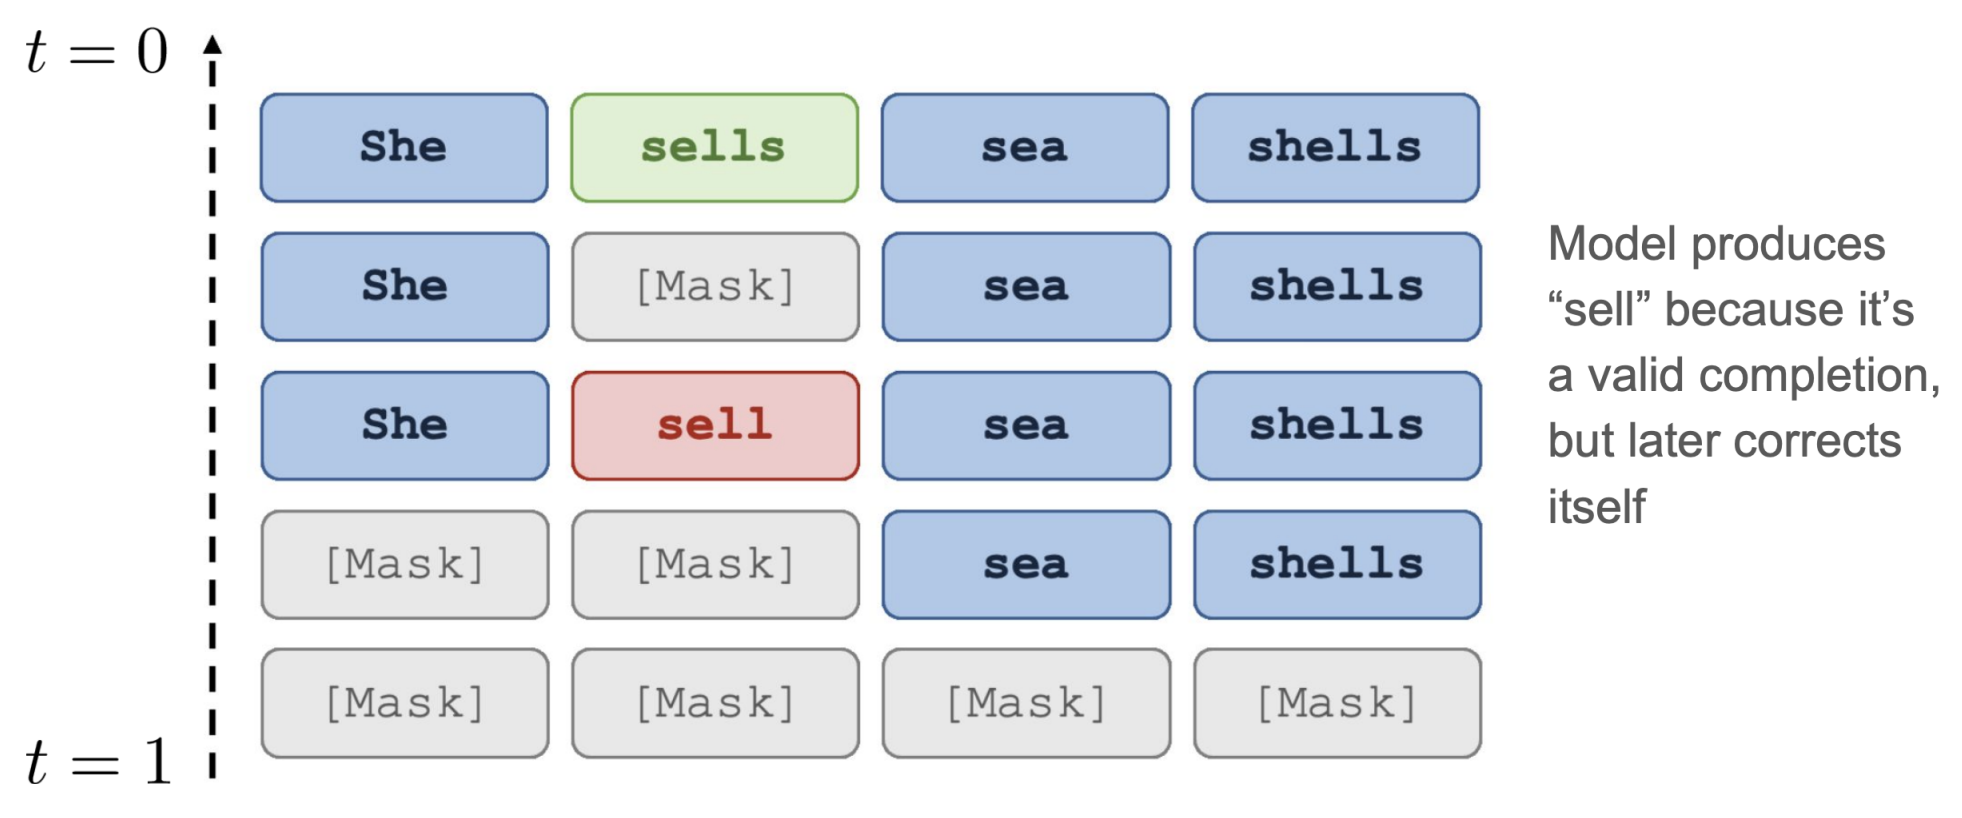
\includegraphics[width=\linewidth]{figure/remasking.png}
\vfill

\end{frame}

\begin{frame}{Prompting With MDLMs}
\vfill
\centering
\medskip
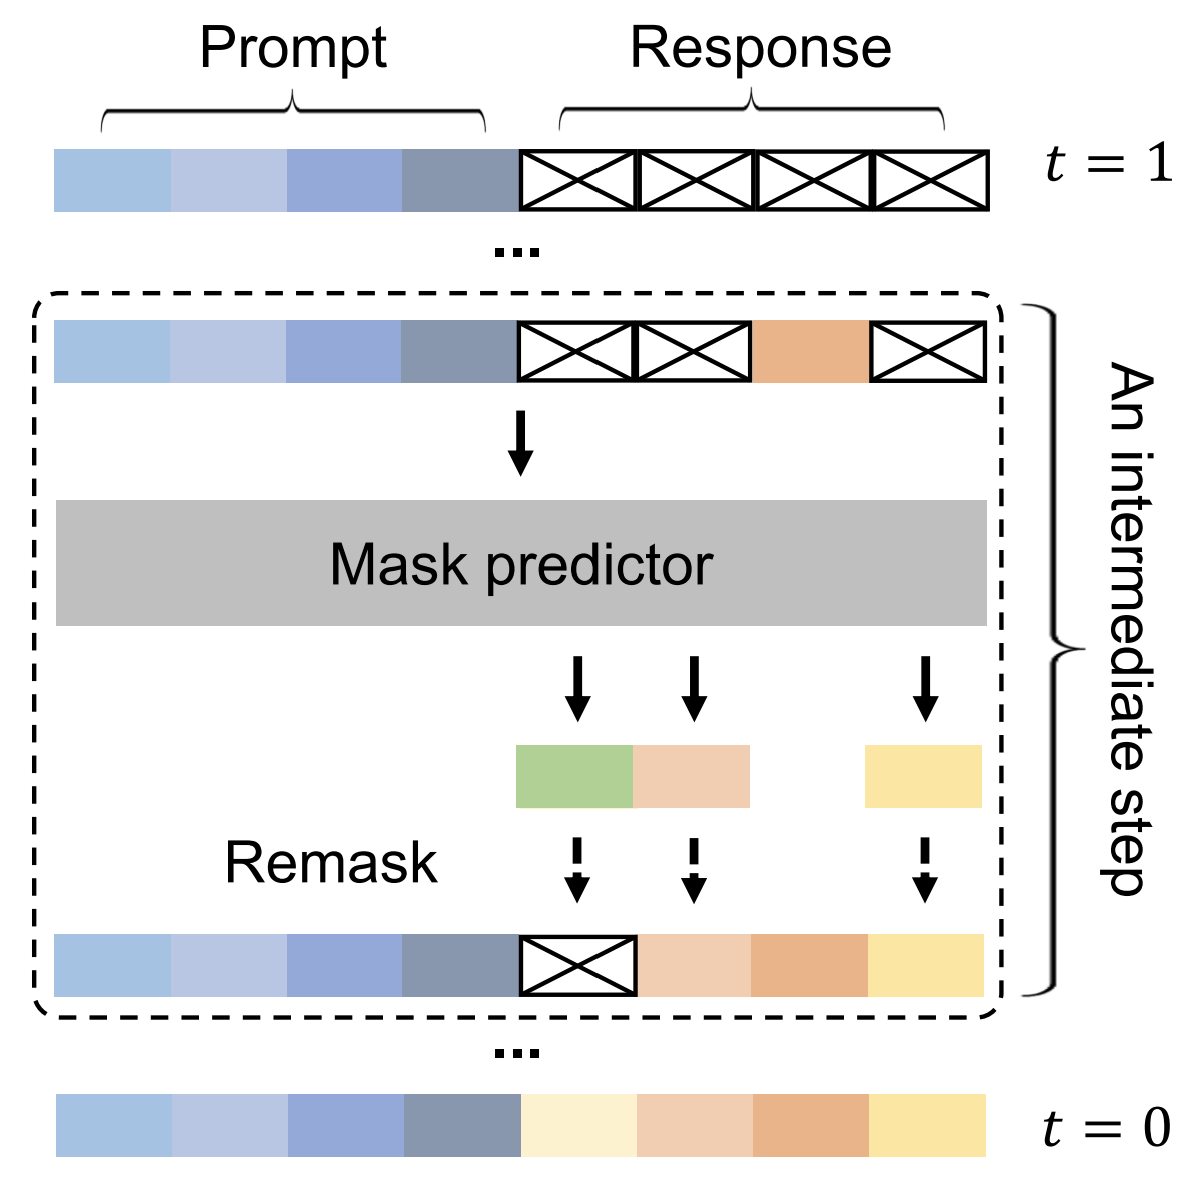
\includegraphics[width=0.6\linewidth]{figure/prompting.png}
\vfill

\end{frame}


\begin{frame}{Alternatives to Masked Diffusion}
\vfill
\centering
\medskip
\medskip
\medskip
\medskip
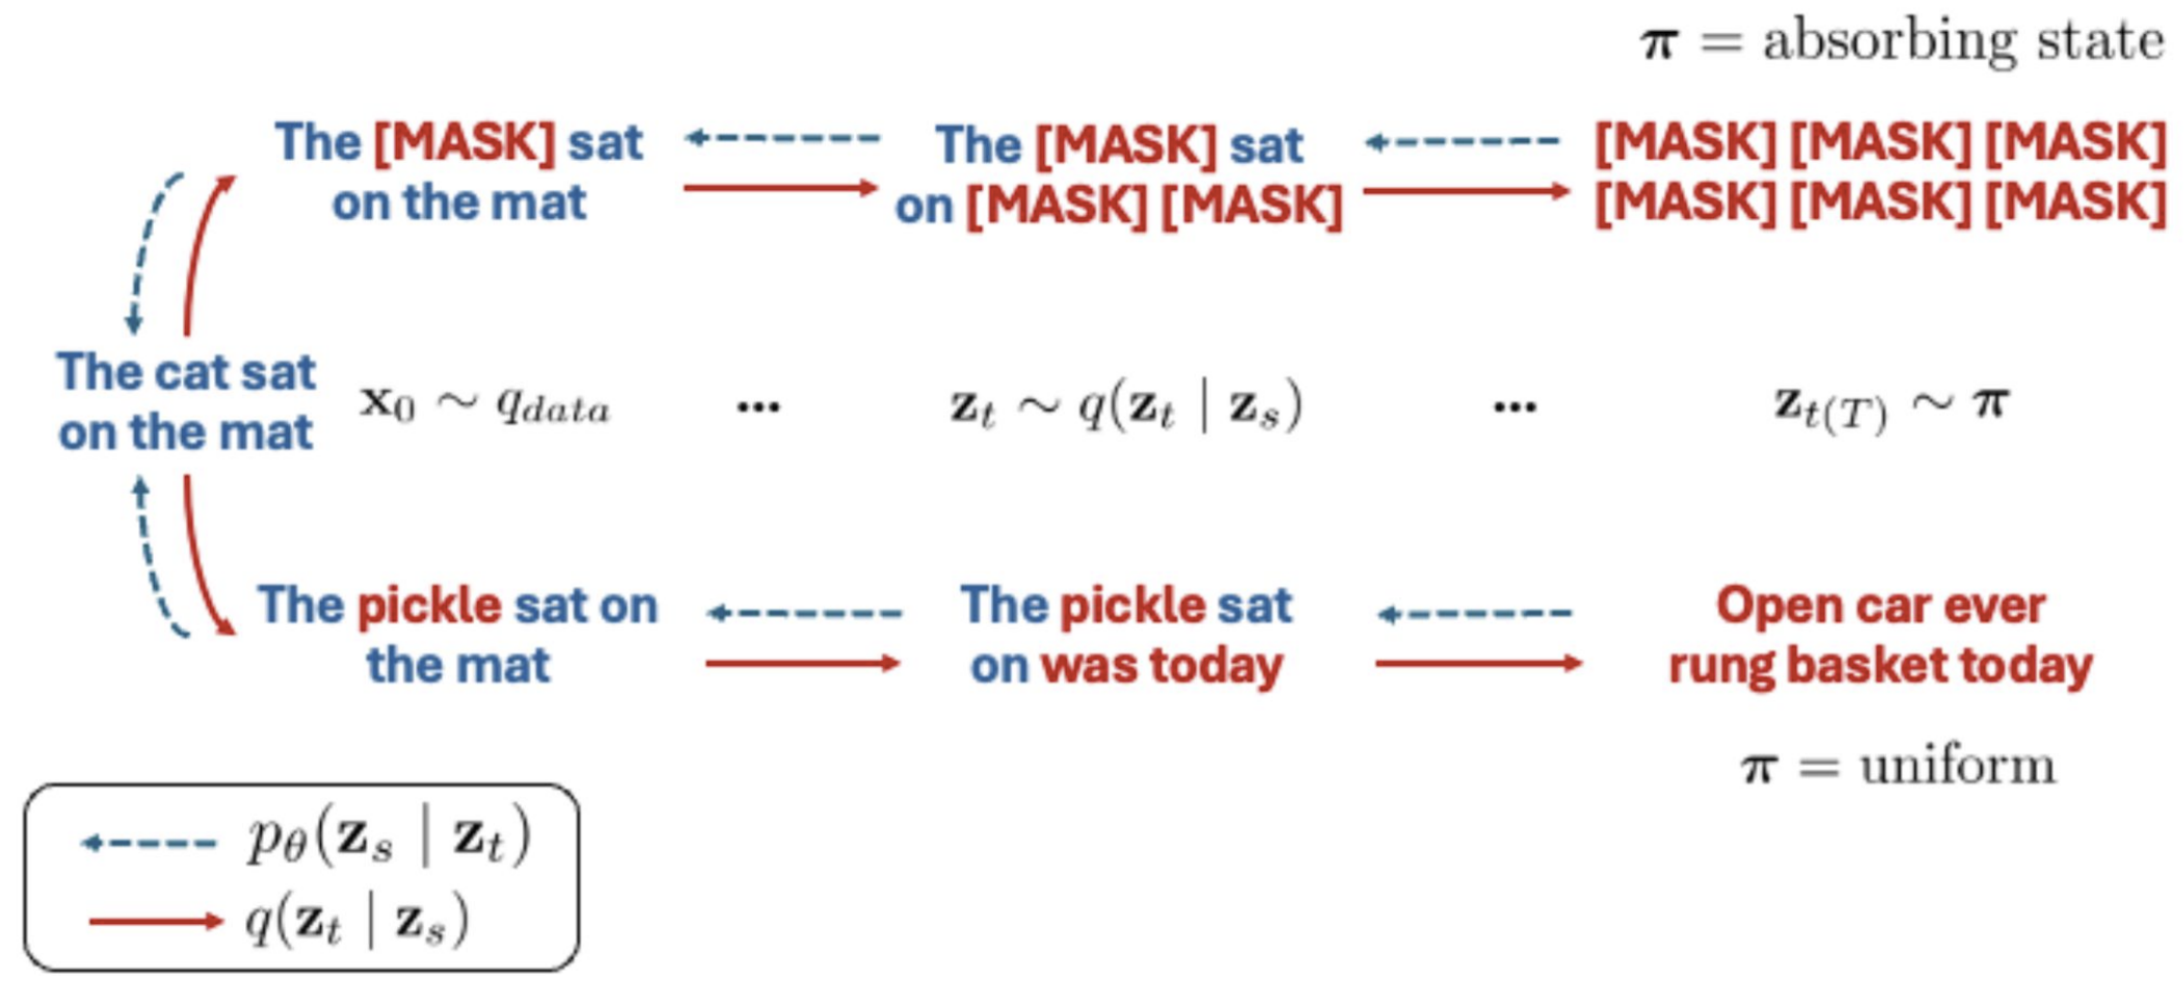
\includegraphics[width=\linewidth]{figure/uniform.png}
\vfill

\end{frame}


\begin{frame}{Very Active Research Area}
\vfill
\centering
\medskip
\medskip
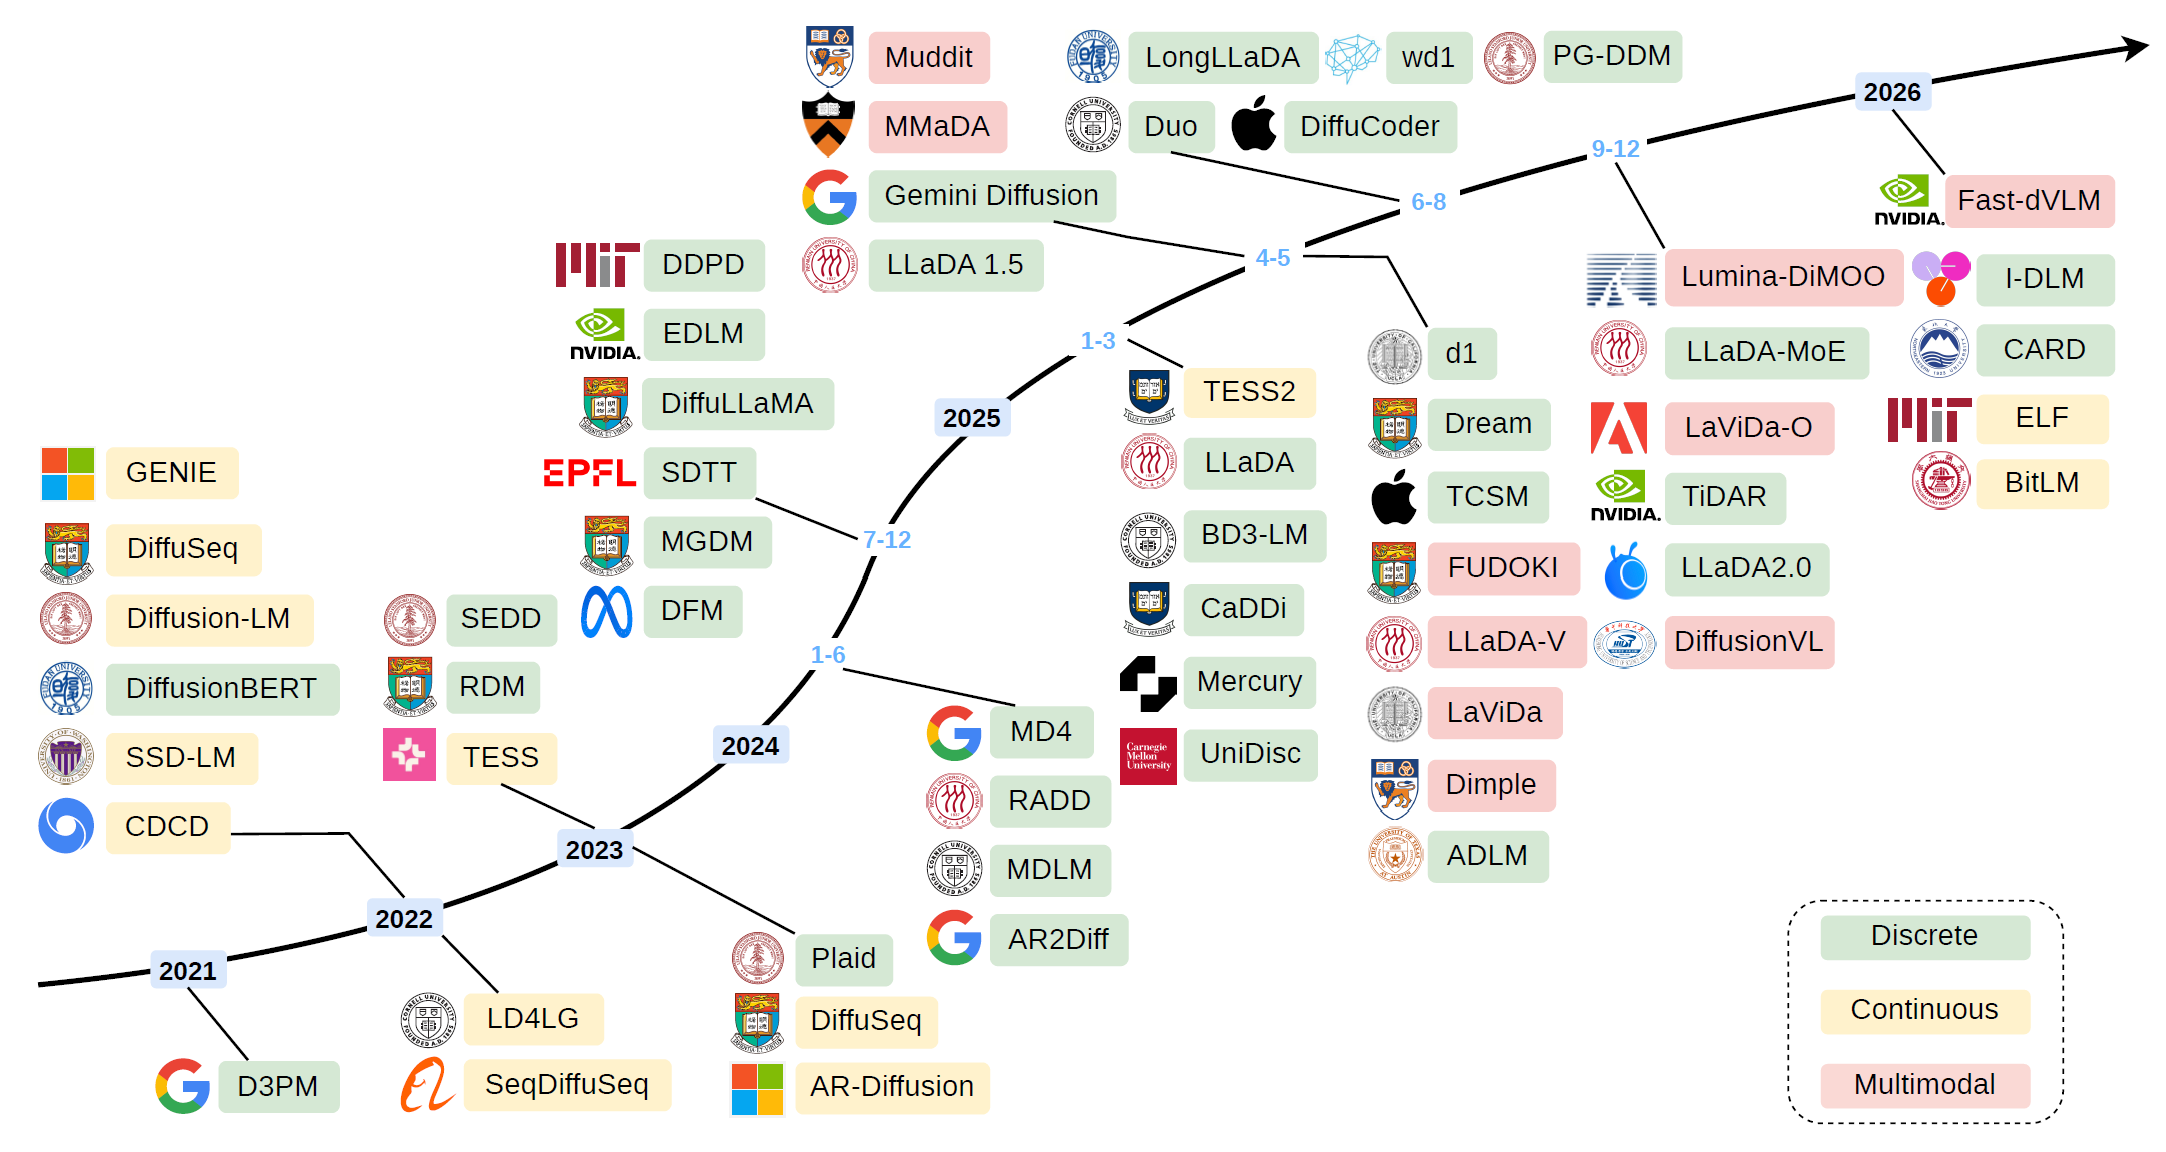
\includegraphics[width=\linewidth]{figure/dlms.png}
\vfill

\end{frame}
 
 

\begin{frame}[allowframebreaks,noframenumbering,plain]{References}
        \tiny
        \bibliographystyle{plain} %apalike
        \bibliography{refs-diffusion}
\end{frame}

\endlecture
\end{document}
